当决定为我应用程序使用FPGA是,或者决定尝试一下FPGA,了解如何编写代码以获得良好的性能很重要。本节会来了解一些重要概念,并涵盖一些常引起混淆的主题,以便更快入门。\par

\hspace*{\fill} \par %插入空行
\textbf{并行性}

我们已经了解了如何使用流水线并行在FPGA上有效地执行工作。另一个简单的流水线示例如图17-12所示。\par

\hspace*{\fill} \par %插入空行
图17-12 具有5个阶段的简单管道:6个时钟周期来处理一个数据元素
\begin{center}
	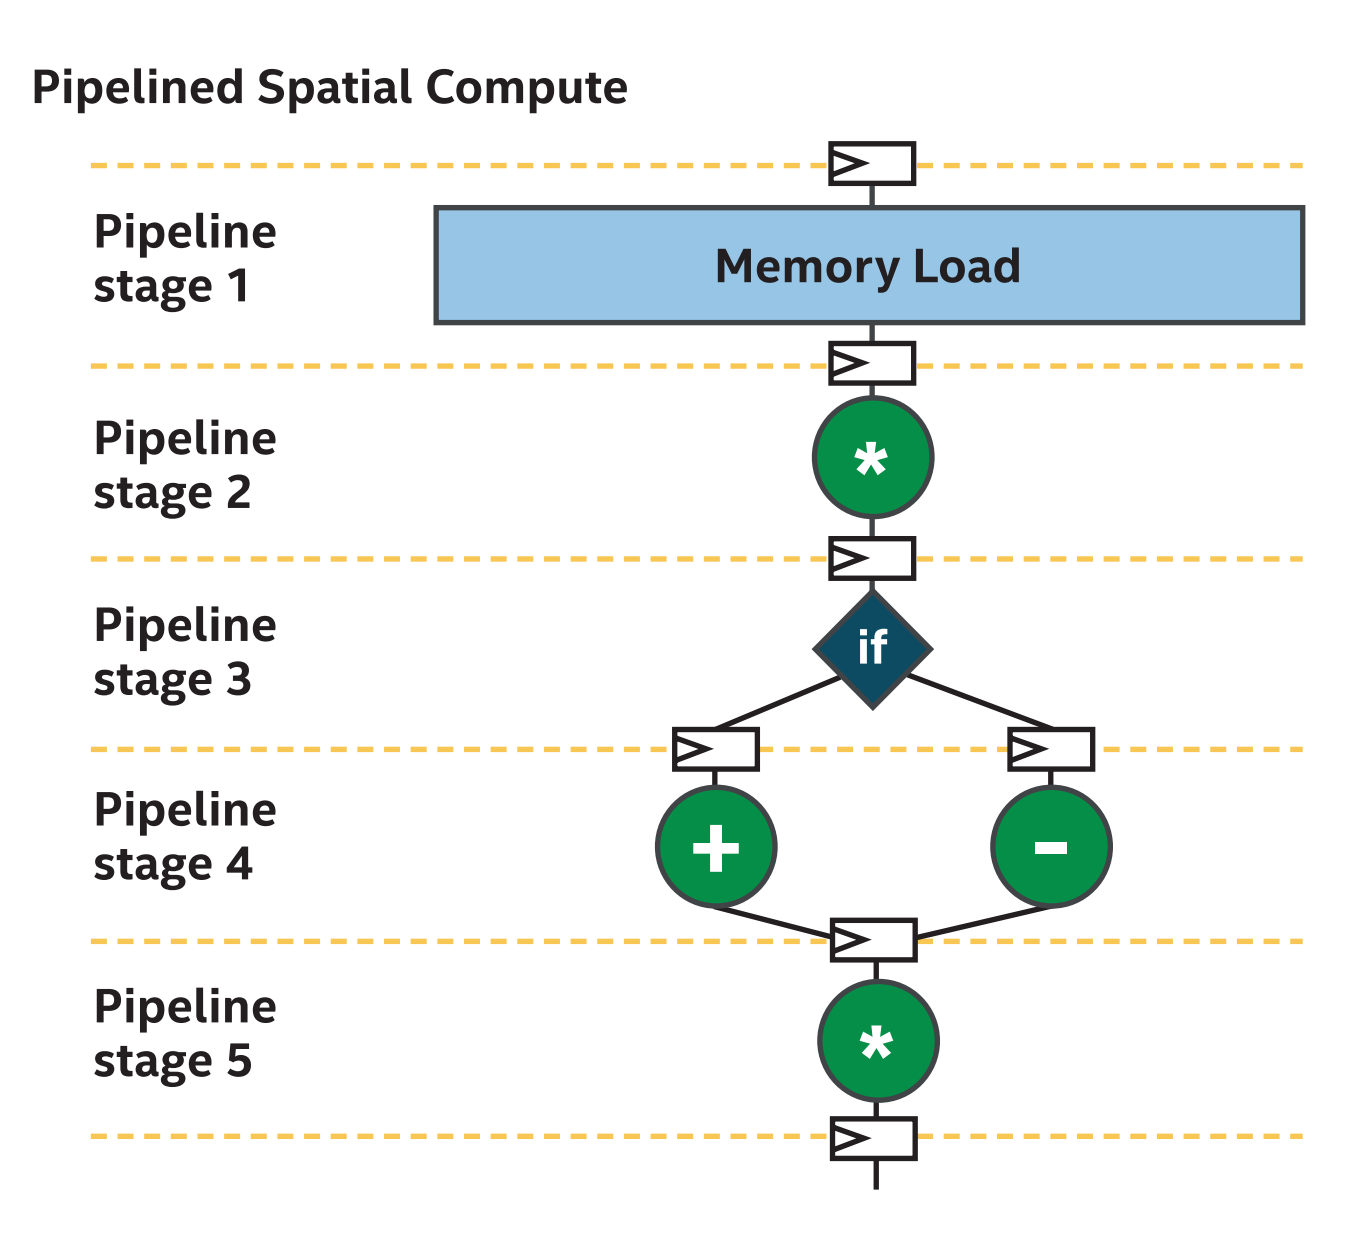
\includegraphics[width=1.0\textwidth]{content/chapter-17/images/11}
\end{center}

在这个过程中,有5个阶段。数据在每个时钟周期中从一个阶段移动到下一个阶段,所以在这个非常简单的例子中,从数据进入阶段1到从阶段5退出需要6个时钟周期。\par

流水线的主要目标是使多个数据元素能够在不同阶段同时处理。为了明确这一点,图17-13展示了一个没有饱和工作(在本例中只有一个数据元素)的管道,这导致在大多数时钟周期中每个阶段都未使用。因为大多数硬件大部分时间都是空闲的,所以这是对FPGA的资源是一种浪费。\par

\hspace*{\fill} \par %插入空行
图17-13 如果只处理单个工作元素,几乎不使用流水线
\begin{center}
	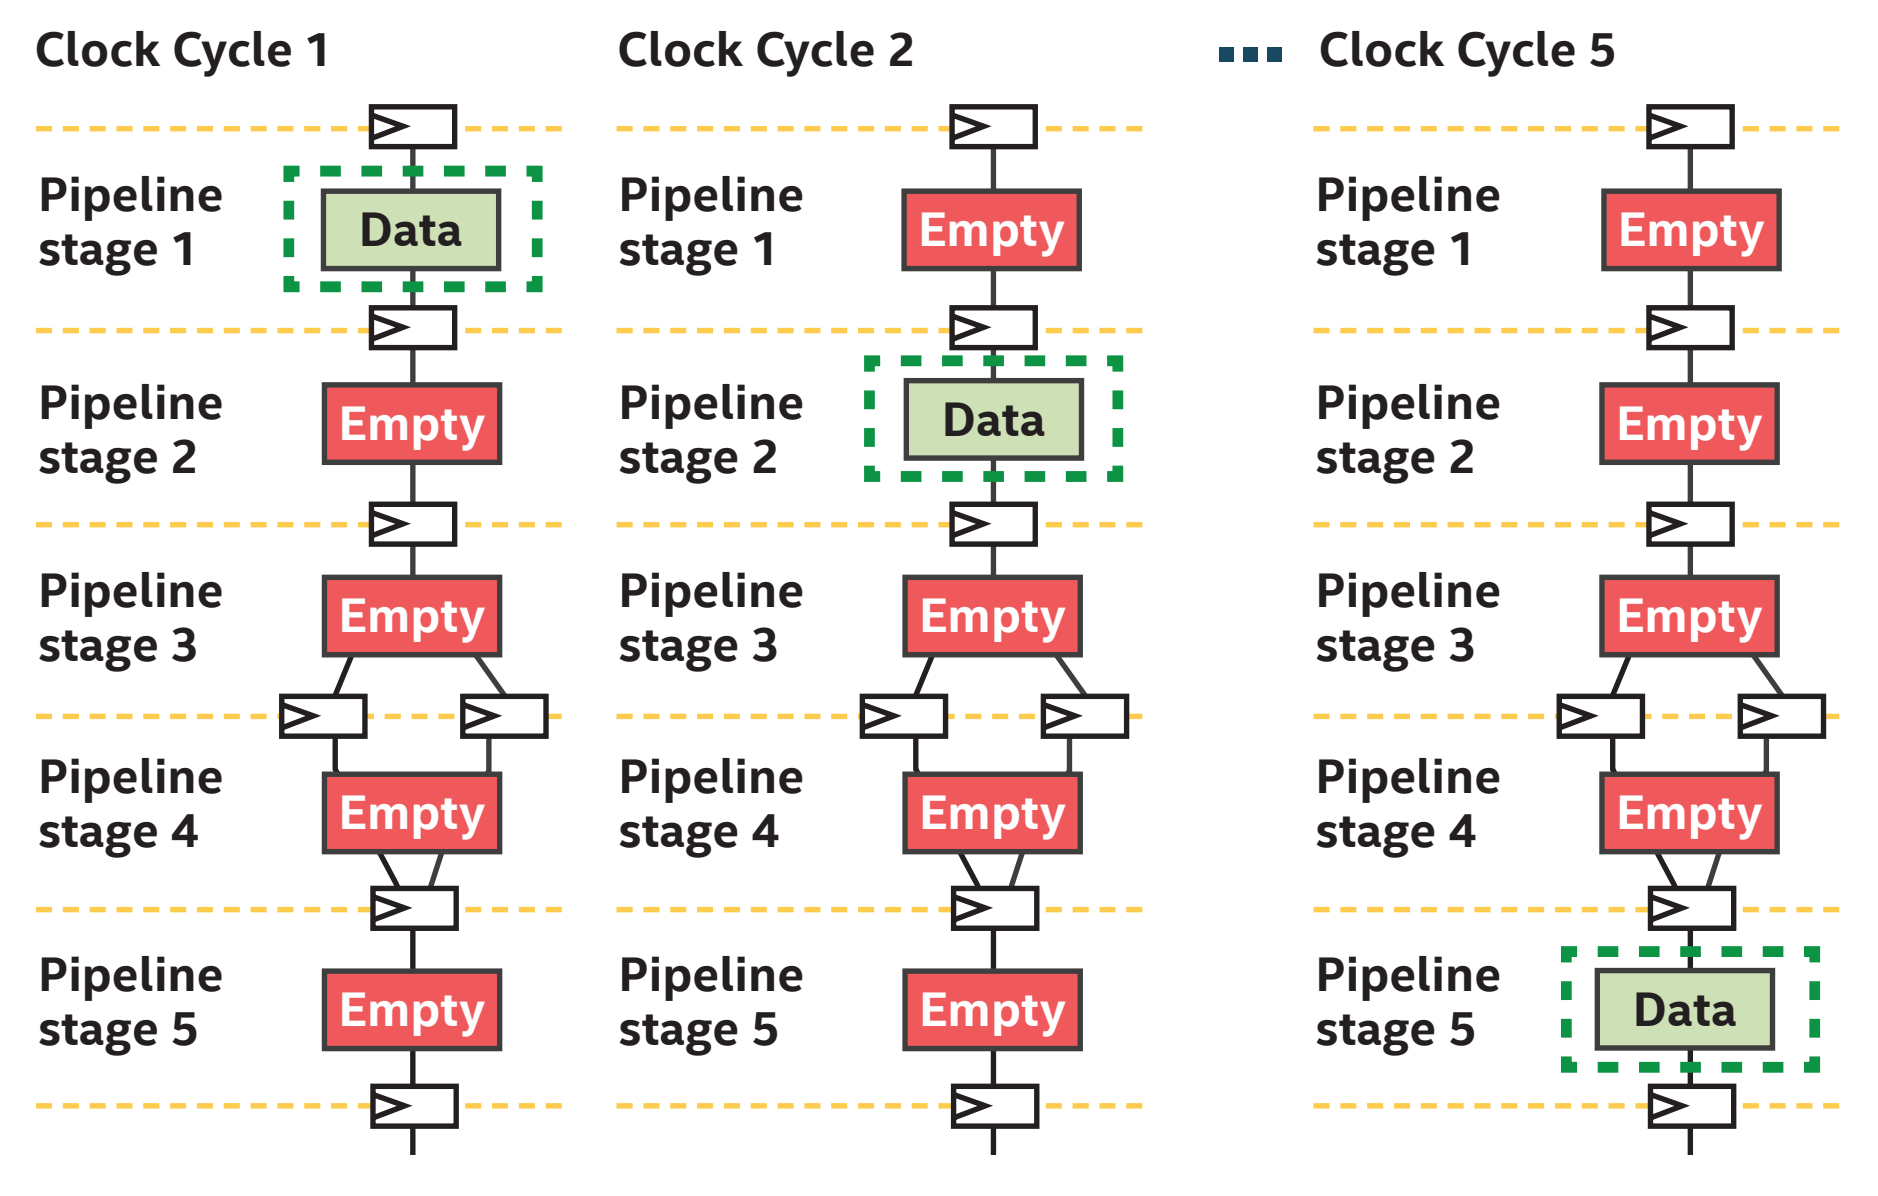
\includegraphics[width=1.0\textwidth]{content/chapter-17/images/12}
\end{center}

为了更好地利用流水线阶段,可以设想在为流水线提供数据的第一个阶段之前,有一个未启动的工作队列等待。每个时钟周期,管道可以从队列中消耗并启动一个工作元素,如图17-14所示。经过一些初始启动周期后,管道的每个阶段都被占用,并在每个时钟周期中做有用的工作,从而使FPGA资源得到有效利用。\par

\hspace*{\fill} \par %插入空行
图17-14 当每个管道阶段都保持忙碌时,就会产生高效的利用
\begin{center}
	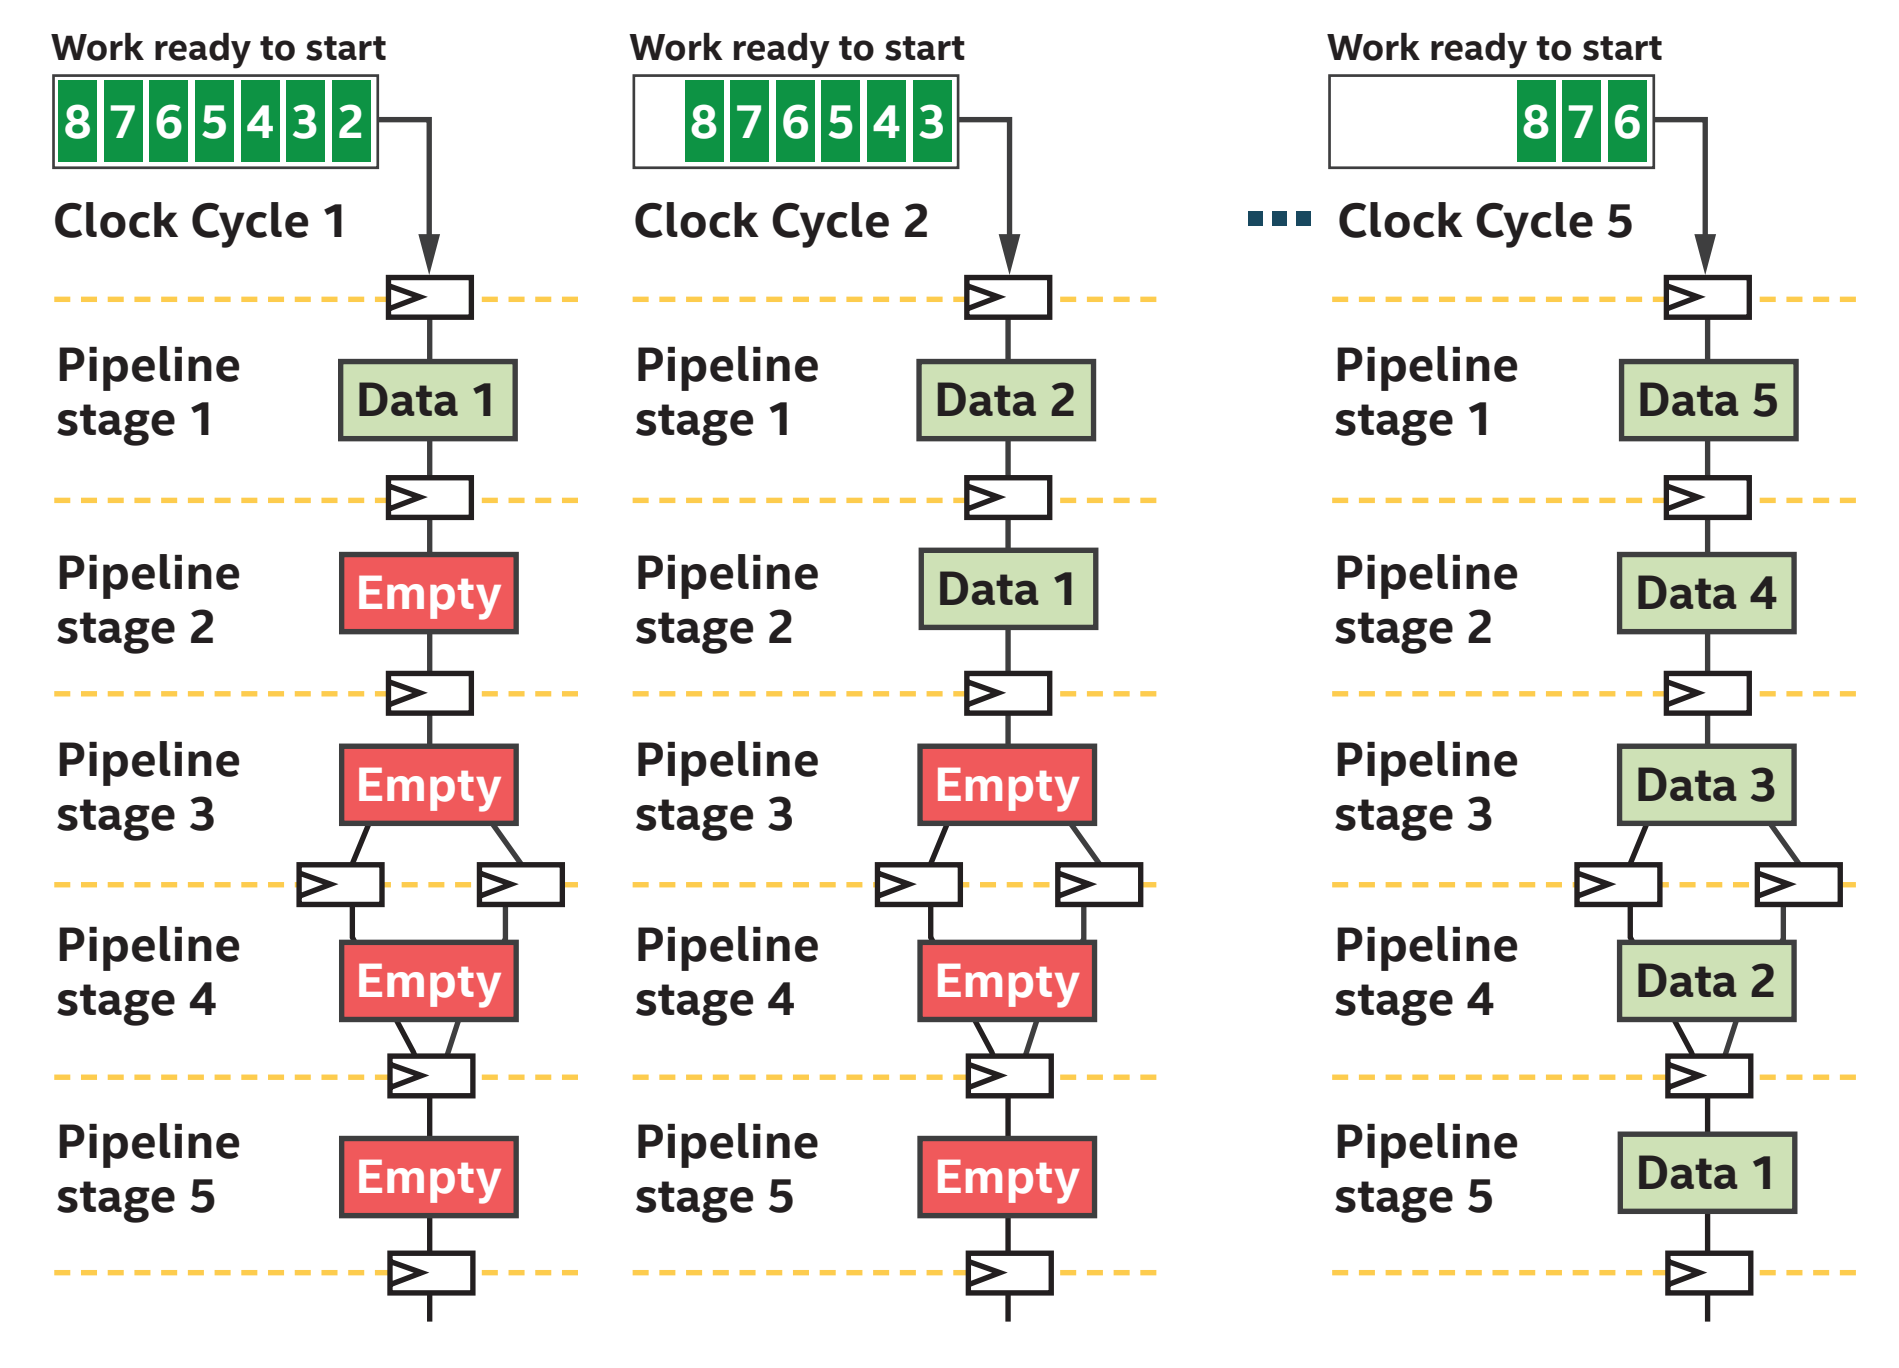
\includegraphics[width=1.0\textwidth]{content/chapter-17/images/13}
\end{center}

下面的两个部分介绍了一些方法,这些方法为队列向流水线输送做启动性工作。我们来看看\par

\begin{enumerate}
	\item ND-range内核
	\item 循环
\end{enumerate}

选择将影响在FPGA上运行的内核的基本架构。某些情况下,算法很适合某种风格,而在其他情况下,开发者的偏好和经验决定了应该选择哪种方法。\par

\hspace*{\fill} \par %插入空行
\textbf{使用ND-Range使流水线繁忙起来}

第4章描述了ND-Range分层执行模型。图17-15说明了关键概念:一个ND-Range执行模型,其中有工作项的分层分组,工作项是内核定义的基本工作单元。这个模型最初是用来来支持GPU的高效编程,其中工作项可以在执行模型层次结构的不同级别上并发执行。为了匹配GPU硬件高效的工作类型,ND-Range工作项在大多数应用程序中相互不通信。\par

\hspace*{\fill} \par %插入空行
图17-15 ND-Range执行模型:工作项的分层分组
\begin{center}
	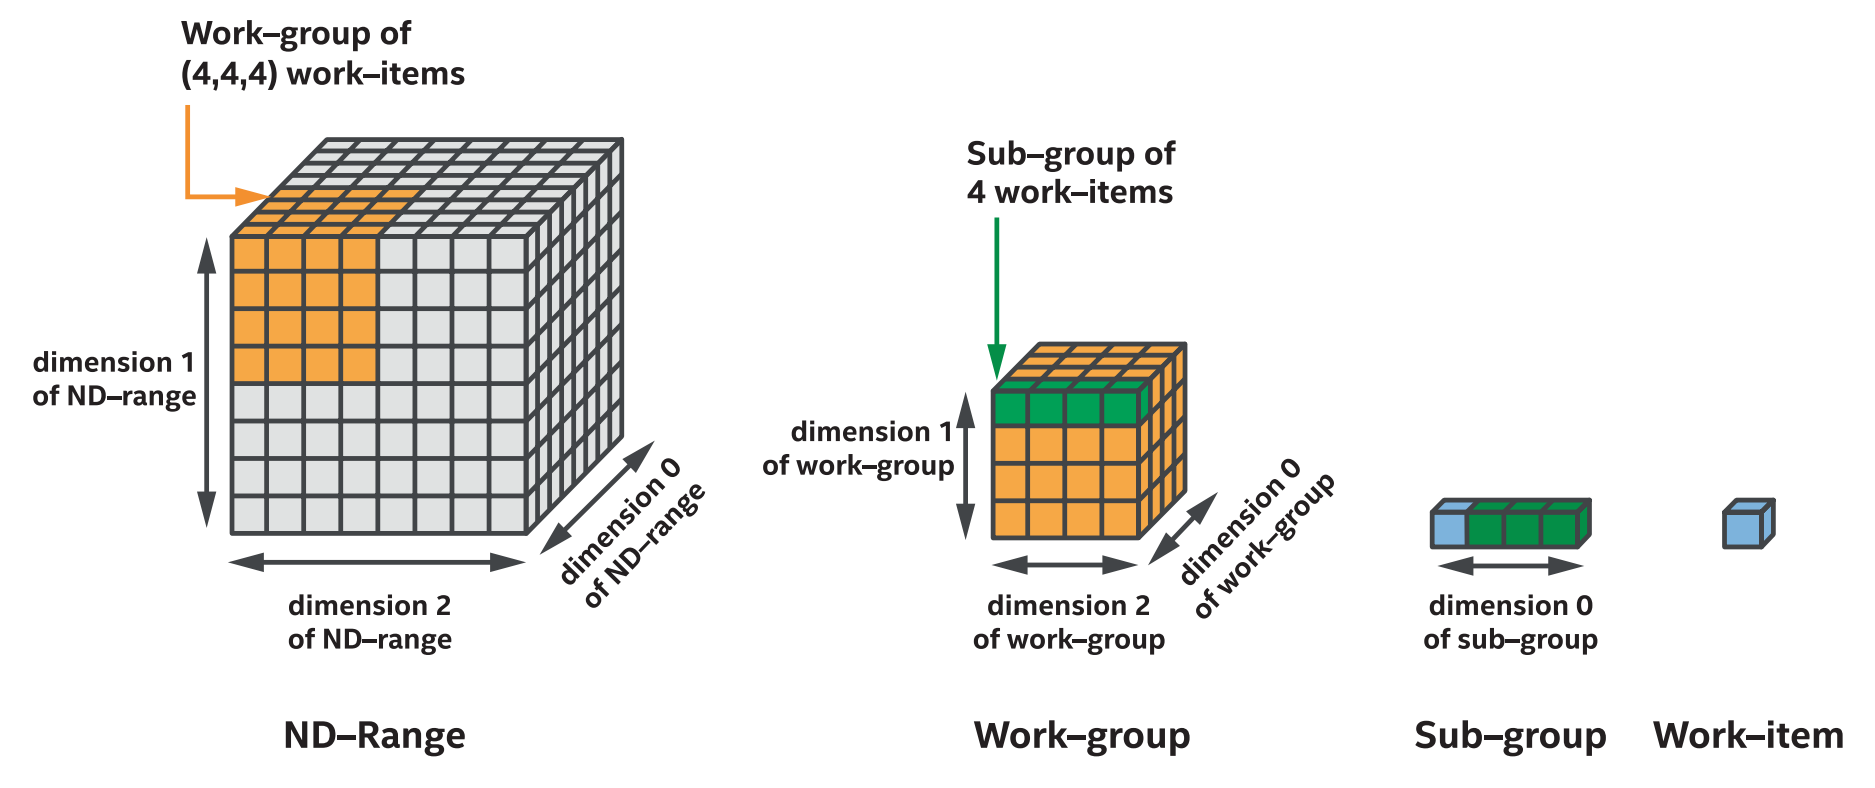
\includegraphics[width=1.0\textwidth]{content/chapter-17/images/14}
\end{center}

FPGA流水线可以非常有效地使用ND-Range进行填充。FPGA完全支持这种编程风格,可以将其看作如图17-16所示,在每个时钟周期上,不同的工作项会进入第一阶段。\par

\hspace*{\fill} \par %插入空行
图17-16 ND-Range向流水线输送任务
\begin{center}
	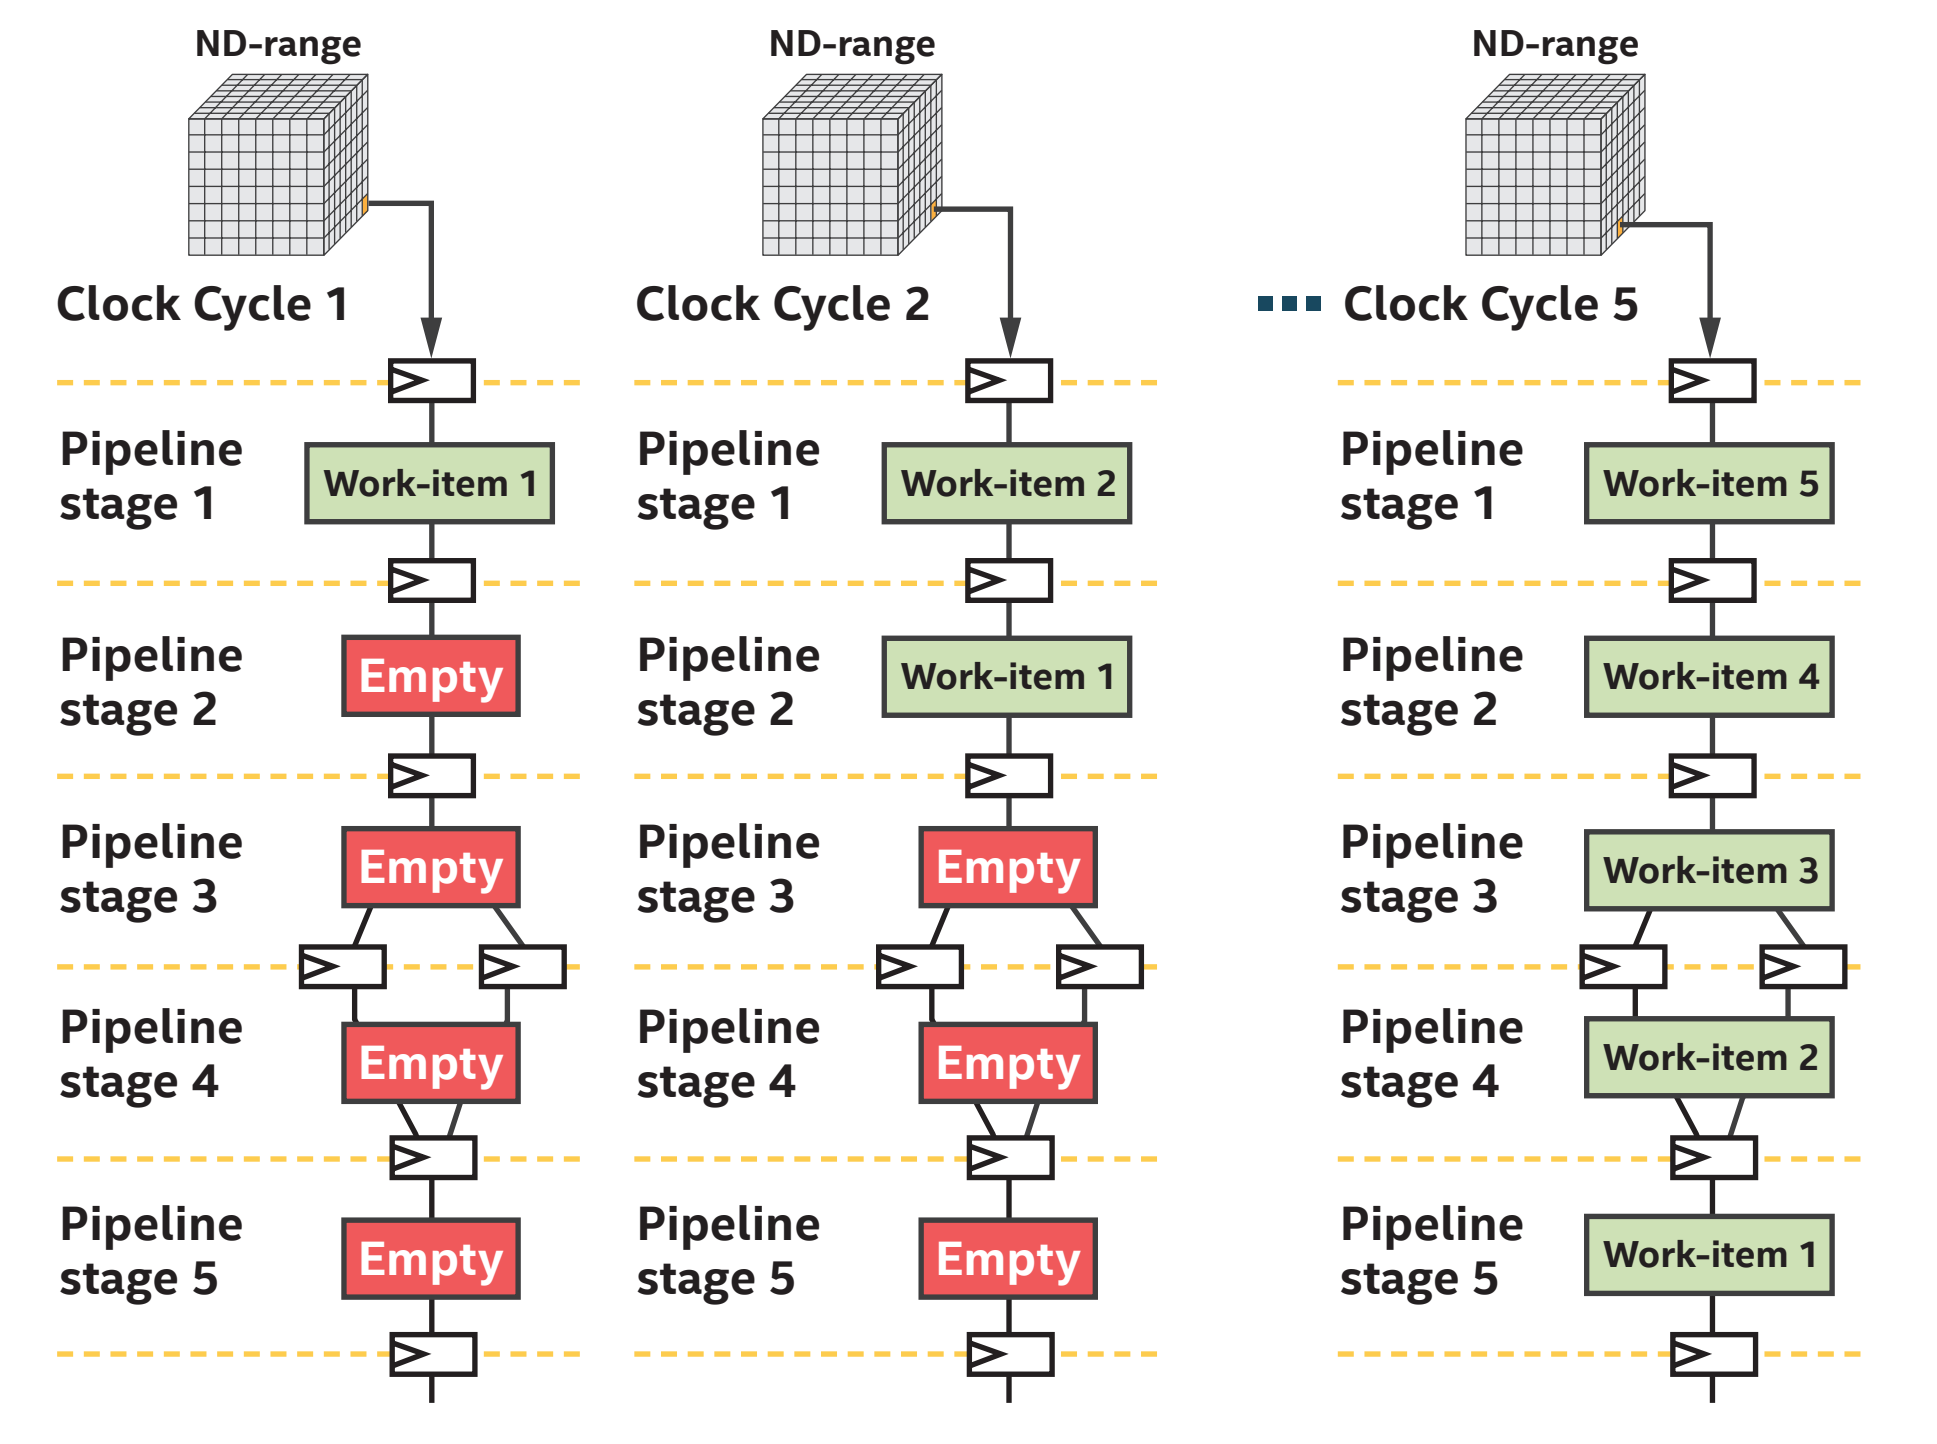
\includegraphics[width=1.0\textwidth]{content/chapter-17/images/15}
\end{center}

什么时候应该使用工作项在FPGA上创建ND-Range内核以保持流水线占用呢?当可以将算法或应用程序构建为独立的工作项,而这些工作项不需要经常通信(或者理想情况下根本不需要交流)时,应该使用ND-Range!如果工作项确实需要经常通信,或者不考虑使用DN-Range,那么循环(在下一节中描述)提供了一种高效的方式来表示我们的算法。\par

\begin{tcolorbox}[colback=red!5!white,colframe=red!75!black]
如果可以构建我们的算法,使工作项不需要太多(或根本不需要)交流,那么ND-Range是生成工作以保持流水线占满的好方法!
\end{tcolorbox}

使用ND-Range输入流水线高效内核的一个例子是随机数生成器,在该序列中创建的数字独立于之前生成的数字。\par

图17-17展示了一个ND-Range内核,它对16×16×16范围内的每个工作项进行了一次随机数生成。注意随机数生成函数如何将工作项id作为输入。\par

\hspace*{\fill} \par %插入空行
图17-17 随机数生成器的多工作项(16 × 16 × 16)
\begin{lstlisting}[caption={}]
h.parallel_for({16,16,16}, [=](auto I) {
	output[I] = generate_random_number_from_ID(I);
});
\end{lstlisting}

示例展示了一个使用range的paralle\_for,只指定了全局大小。可以交替使用带有nd\_range的parallel\_for,其中指定了全局工作大小和本地工作组大小。FPGA可以从片上资源实现工作组本地内存,所以只要有意义就可以随意使用工作组,要么因为想要工作组本地内存,要么因为有可用的工作组id可以简化代码。\par

\begin{tcolorbox}[colback=blue!5!white,colframe=blue!75!black, title=并行随机数生成器]
图17-17中的示例假设generate\_random\_number\_from\_ID(I)是一个随机数生成器,编写为在并行调用时安全且正确。例如,如果parallel\_for内的不同工作项执行这个函数,期望每个工作项创建不同的序列,每个序列都符合生成器所期望的任何分布。并行随机数生成器本身是一个很复杂的主题,因此可以使用库或通过块超前跳过算法等技术了解该主题。
\end{tcolorbox}

\hspace*{\fill} \par %插入空行
\textbf{流水线无视数据依赖!}

当一些工作项为向量架构(例如GPU)编程时,一个挑战是在工作项之间没有通信的情况下是一个高效的算法。有些算法和应用程序很适合向量硬件,有些则不行。导致问题的一个常见原因是,由于数据依赖于在某种意义上相邻的其他计算,算法需要共享数据。子工作组通过工作项之间的通信来解决向量体系结构上的挑战,如第14章所述。\par

FPGA对于不能分解成独立工作的算法起着重要的作用。FPGA流水线没有跨工作项进行向量化,而是跨流水线阶段执行连续的工作项。这种并行性的实现,意味着可以在流水线中轻松有效地实现工作项(甚至是不同工作组中的工作项)之间的细粒度通信!\par

例子是随机数生成器它的输出N+1取决于输出N是什么。这在两个输出之间创建了数据依赖关系,如果每个输出都是由ND-Range范围内的工作项生成的,那么工作项之间就存在着数据依赖关系,这可能需要在某些体系结构上进行复杂且通常代价高昂的同步。当按顺序编码这样的算法时,通常会写一个循环,其中迭代N+1使用迭代N的计算,如图17-18所示。每次迭代都依赖于前一次迭代计算的状态。\par

\hspace*{\fill} \par %插入空行
图17-18 携带数据依赖(状态)的循环
\begin{lstlisting}[caption={}]
int state = 0;
for (int i=0; i < size; i++) {
	state = generate_random_number(state);
	output[i] = state;
}
\end{lstlisting}

该方法可以非常有效地将结果向后传递到后续循环中开始工作的流水线中,和空间编译器实现围绕此模式的许多优化。图17-19展示了从第5阶段到第4阶段的数据反向通信的思想。空间管道不会跨工作项向量化。通过在管道中向后传递结果,支持高效的数据依赖通信!\par

\hspace*{\fill} \par %插入空行
图17-19 向后通信使高效的数据依赖成为可能
\begin{center}
	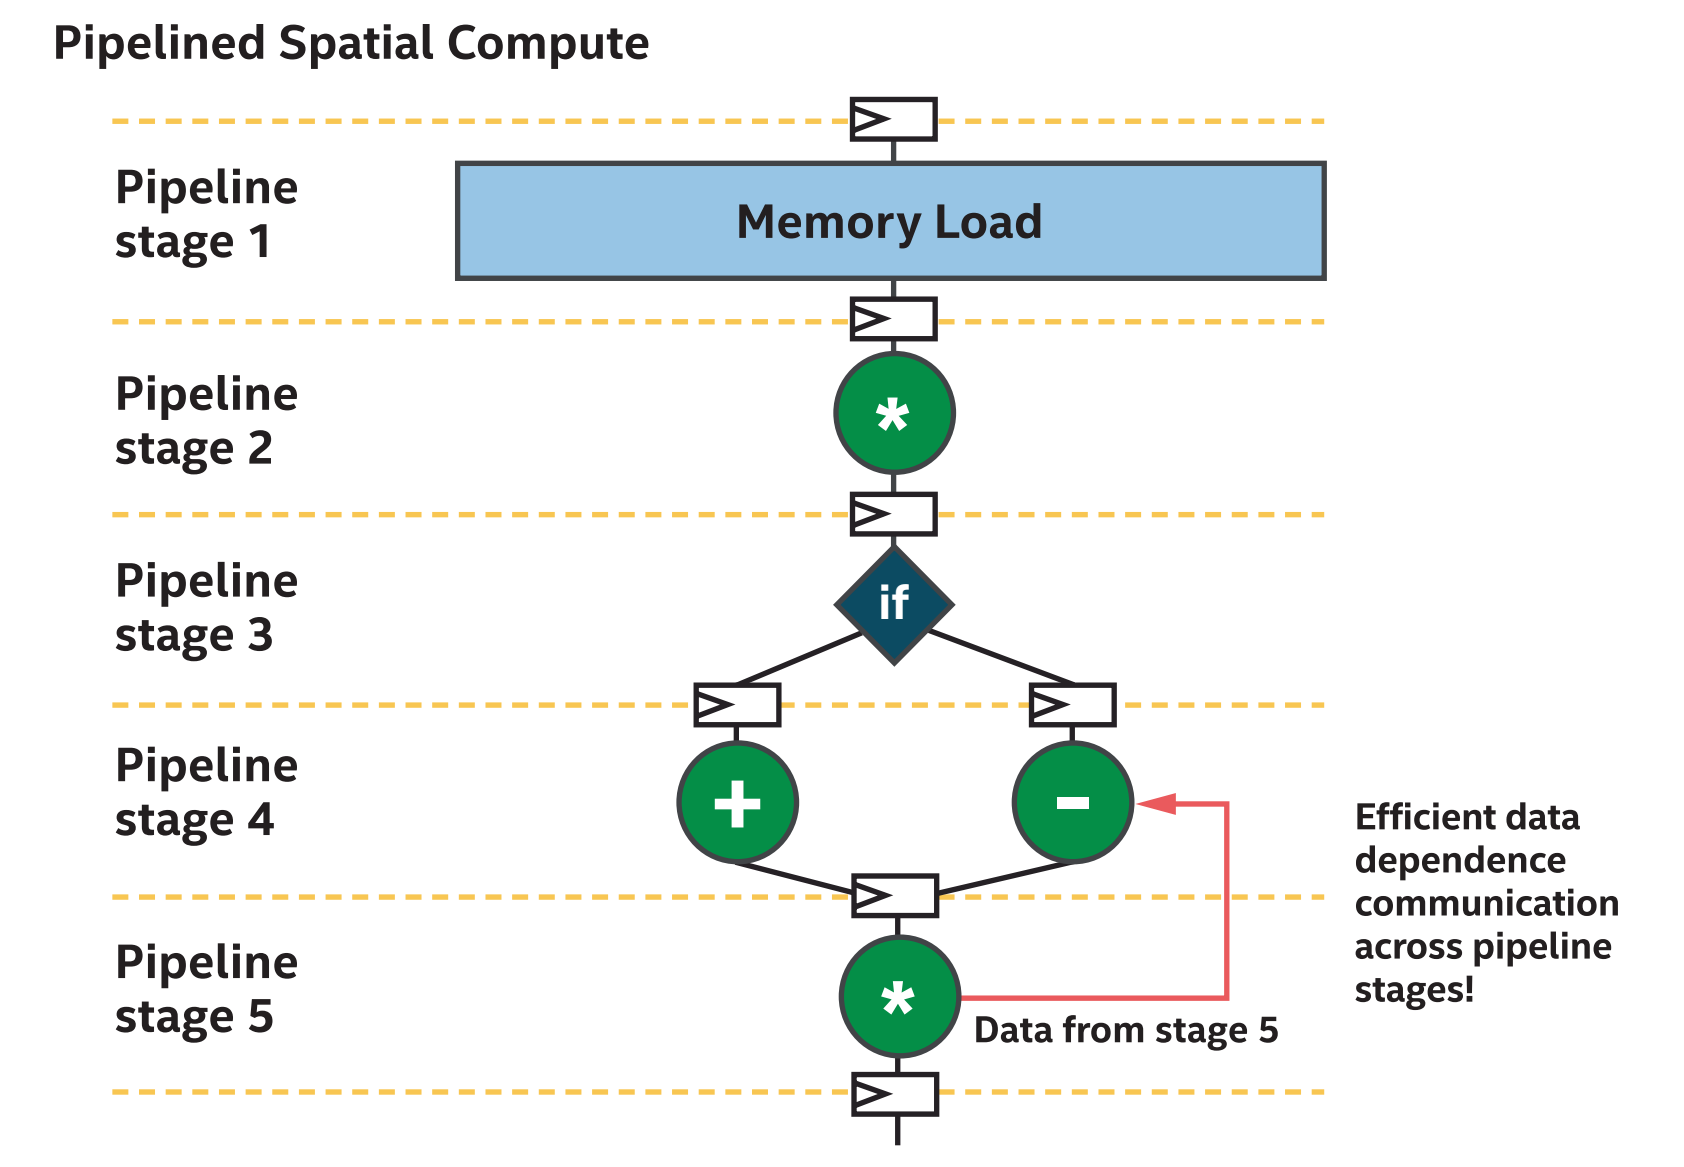
\includegraphics[width=1.0\textwidth]{content/chapter-17/images/16}
\end{center}

向后传递数据(到管道中的早期阶段)的能力是空间体系结构的关键,但是不清楚如何编写利用它的代码。有两种方法可以简化这种模式的表达:有两种方法可以简化这种模式的表达:\par

\begin{enumerate}
	\item 循环
	\item 带有内部管道的ND-Range内核
\end{enumerate}

第二个选项是基于管道的,我们将在本章后面描述它。供应商文档提供了关于管道方法的更多细节,但是常用的还是循环,除非有其他原因。\par

\hspace*{\fill} \par %插入空行
\textbf{空间流水线循环的实现}

当编写具有数据依赖性的算法时,循环是一种自然的选择。循环经常表示迭代之间的依赖关系,即使在最基本的循环示例中,决定循环何时退出的计数器也会在迭代中执行(图17-20中的变量i)。\par

\hspace*{\fill} \par %插入空行
图17-20 带有两个循环依赖项(即i和a)的循环
\begin{lstlisting}[caption={}]
int a = 0;
for (int i=0; i < size; i++) {
	a = a + i;
}
\end{lstlisting}

图17-20的简单循环中,a= a + i右边的a的值反映了前一次循环中存储的值,如果是第一次循环,则是初始值。当空间编译器实现循环时,可以使用循环的迭代来填充管道的各个阶段,如图17-21所示。请注意,现在准备开始的工作队列包含循环迭代,而不是工作项!\par

\hspace*{\fill} \par %插入空行
图17-21 流水线阶段由循环的连续迭代提供
\begin{center}
	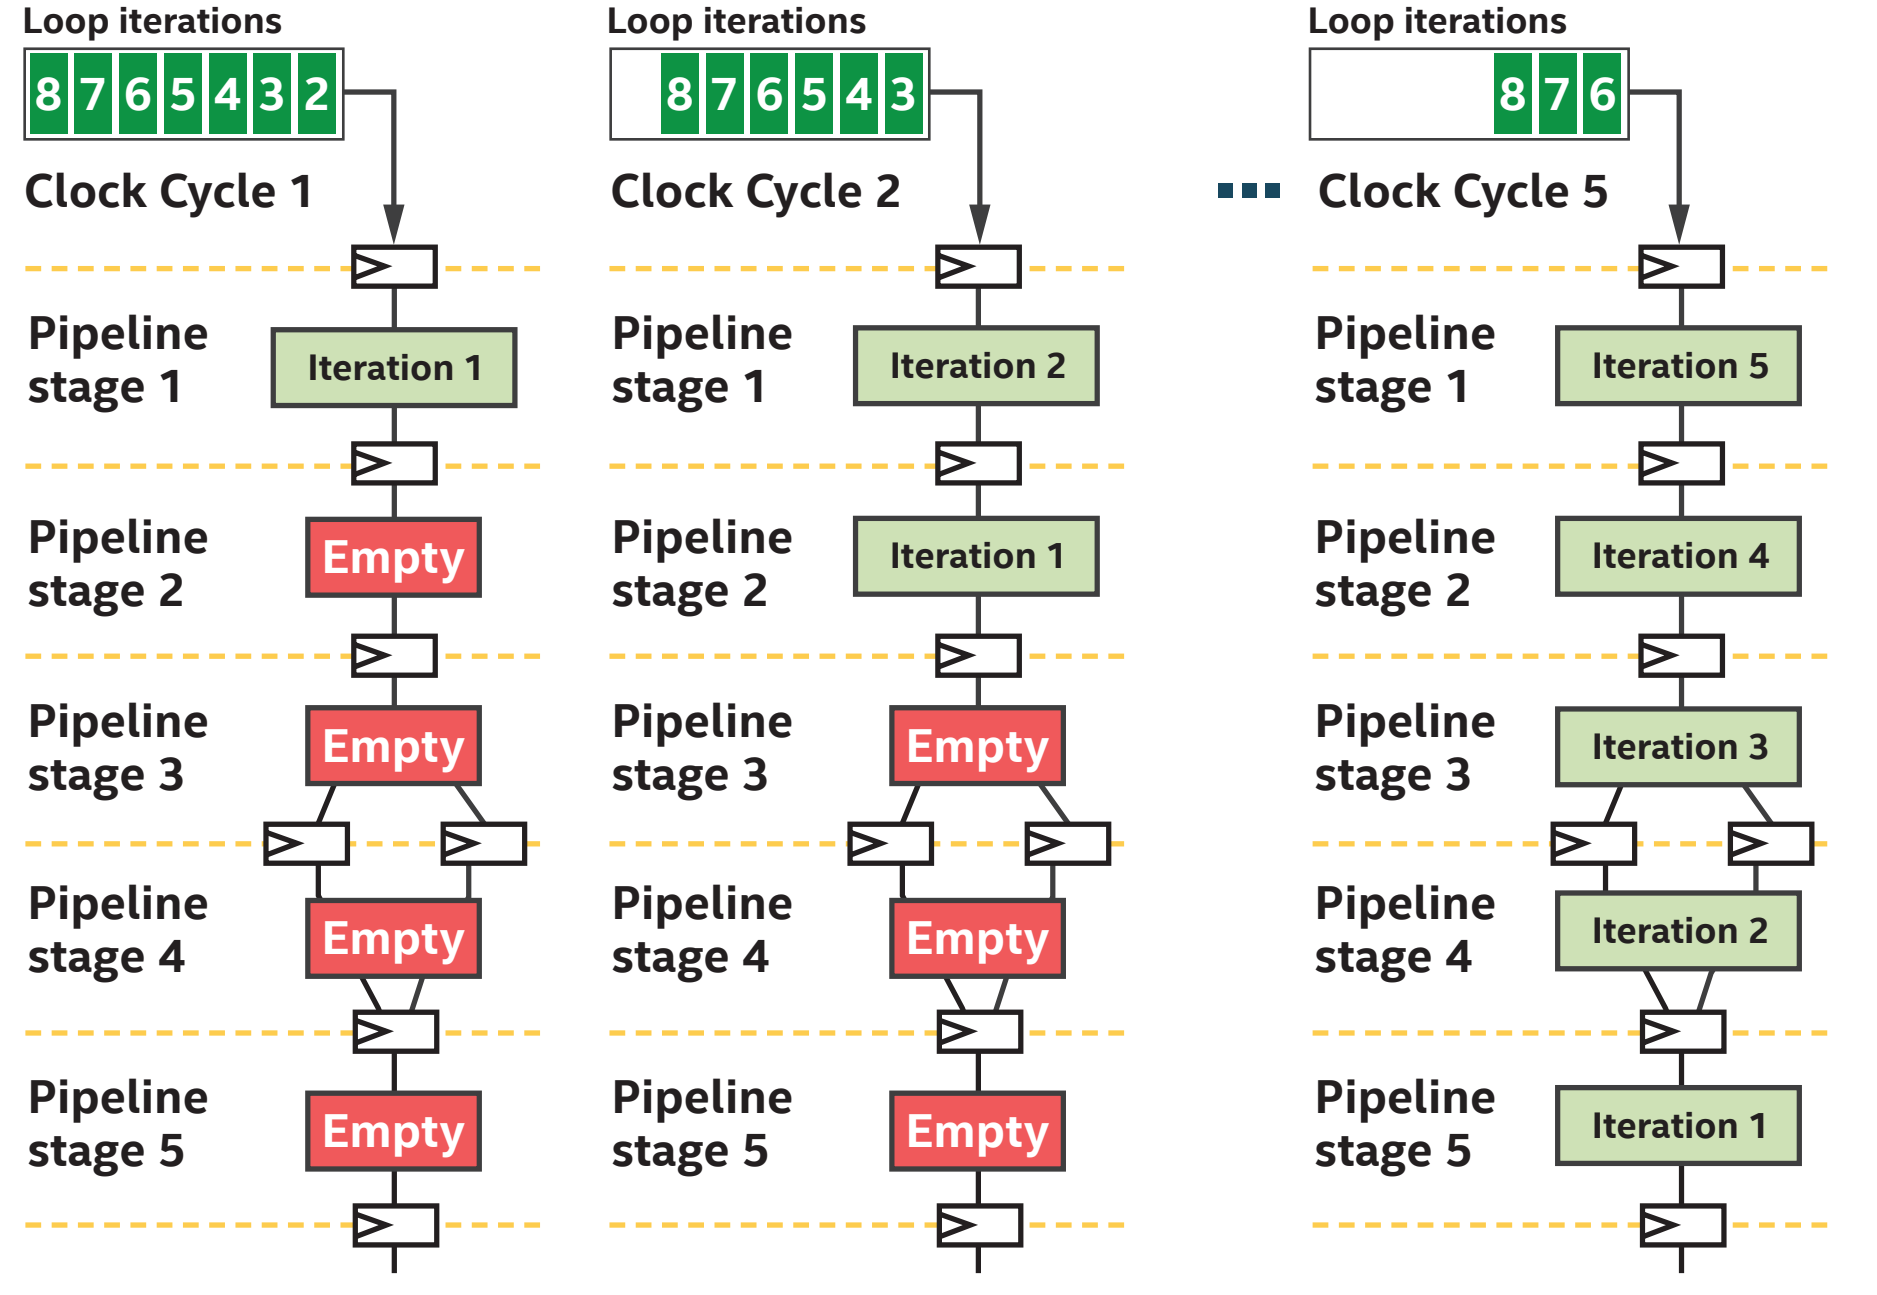
\includegraphics[width=1.0\textwidth]{content/chapter-17/images/17}
\end{center}

修改后的随机数生成器示例如图17-22所示。与基于工作项的id生成数字不同,如图17-17所示,生成器将先前计算的值将作为参数。\par

\hspace*{\fill} \par %插入空行
图17-22 依赖于之前生成的值的随机数生成器
\begin{lstlisting}[caption={}]
h.single_task([=]() {
	int state = seed;
	for (int i=0; i < size; i++) {
		state = generate_incremental_random_number(state);
		output[i] = state;
	}
});
\end{lstlisting}

这个例子使用了single\_task而不是paralle\_for,因为重复的工作是通过单个任务中的循环来表示,所以没有理由在此代码中还包含多个工作项(通过parallel\_for)。single\_task内部的循环使得将之前计算的temp值传递给随机数生成函数的每次使用更加容易(编程方便)。\par

如图17-22所示的情况下,FPGA可以有效地实现环路。许多情况下,它可以保持流水线完全占用的状态,或者至少可以通过报告告诉我们应该改变什么来增加占用率。考虑到这一点,如果循环迭代被工作项取代,那么同样的算法将更加难以描述,其中由一个工作项生成的值将需要传递给在增量计算中使用的另一个工作项。代码复杂性将迅速增加,特别是如果工作不能进行批处理,使每个工作项实际计算自己独立的随机数序列。\par

\hspace*{\fill} \par %插入空行
\textbf{循环起始的间隔}

从概念上讲,认为C++中的循环迭代是一个接一个地执行,如图17-23所示。这是编程模型,也是思考循环的正确方式。实际中,编译器可以执行许多优化,只要程序的大部分行为(即定义的和无种族行为)没有明显的变化。不管编译器的优化如何,重要的是循环的执行看起来就像图17-23所示的那样。\par

\hspace*{\fill} \par %插入空行
图17-23 从概念上讲,循环迭代一个接一个地执行
\begin{center}
	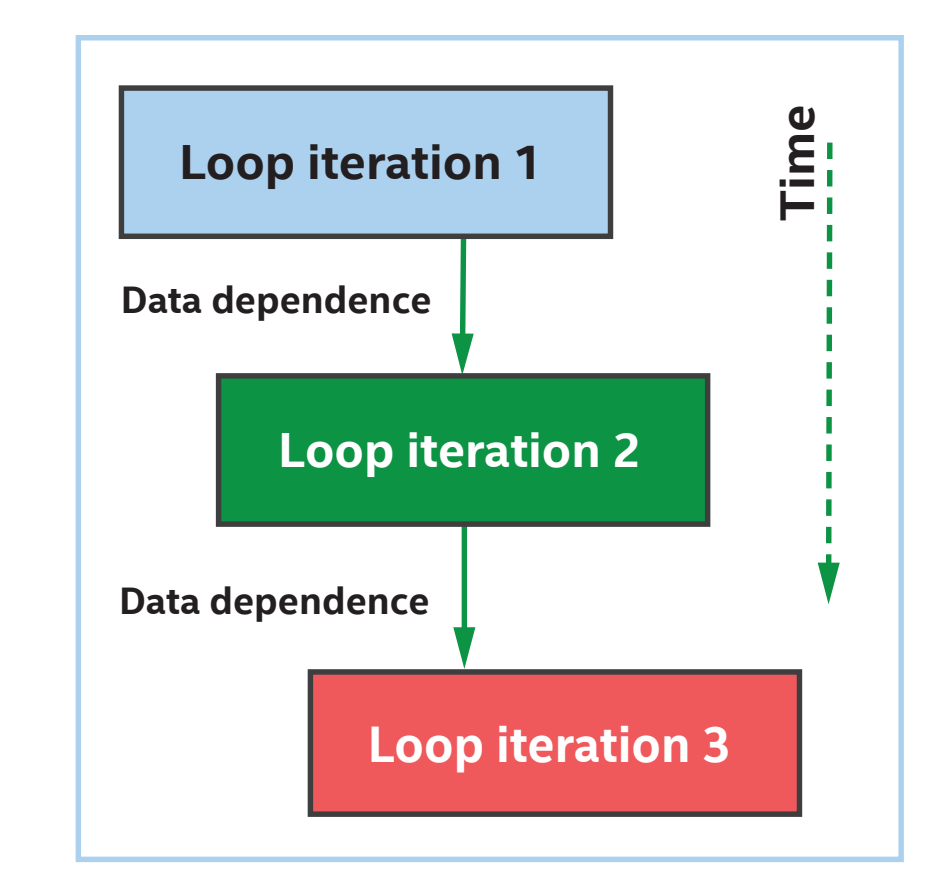
\includegraphics[width=1.0\textwidth]{content/chapter-17/images/18}
\end{center}

进入空间编译器透视图,图17-24显示了一个循环流水线优化,其中循环迭代的执行在时间上是重叠的。不同的迭代将彼此执行流水线的不同阶段,而各个阶段的数据依赖可以由编译器管理,以确保程序执行的迭代好似是顺序的(除了循环将更快地完成执行)。\par

\hspace*{\fill} \par %插入空行
图17-24 循环流水线允许循环的迭代在流水线阶段之间重叠
\begin{center}
	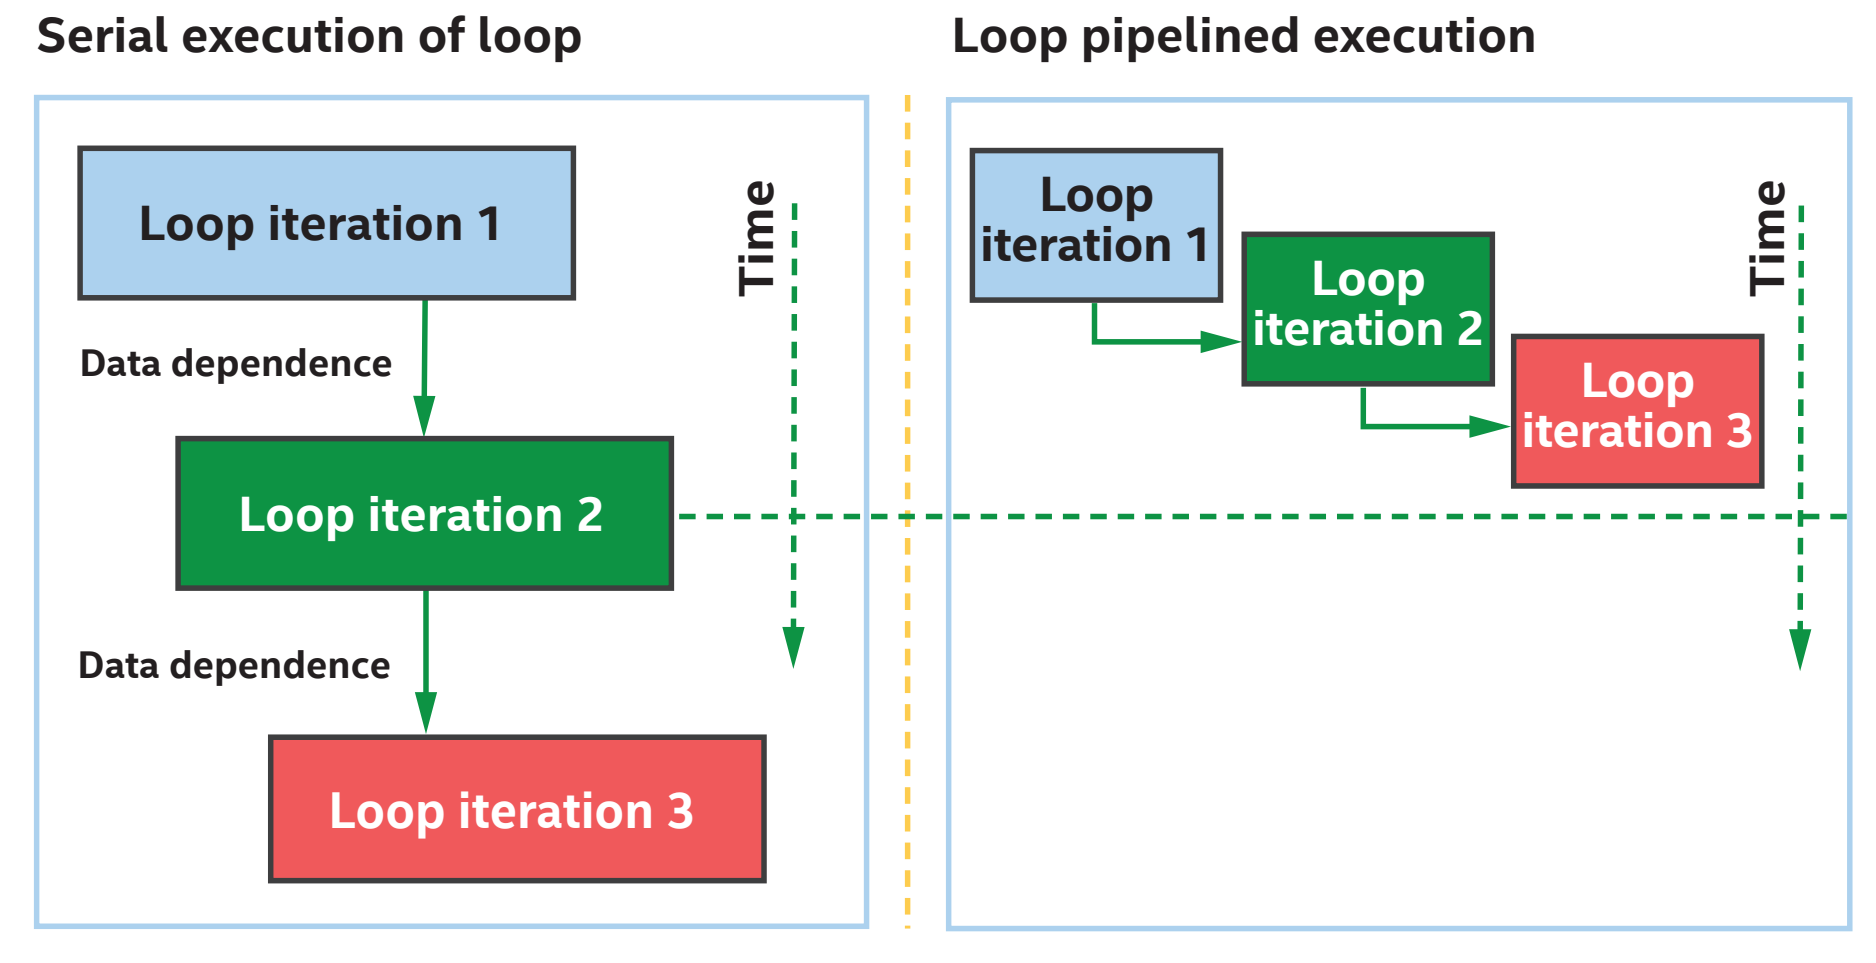
\includegraphics[width=1.0\textwidth]{content/chapter-17/images/19}
\end{center}

在流水线中,当编译器决定这样做时,结果可以传递到更早的阶段,这样,循环迭代中的许多结果可能在循环迭代完成所有工作之前就完成了计算。图17-25展示了这种思想,阶段1的结果在管道中向后反馈,允许未来的循环迭代在前一个迭代完成之前使用结果。\par

\hspace*{\fill} \par %插入空行
图17-25 增量随机数生成器的流水线实现
\begin{center}
	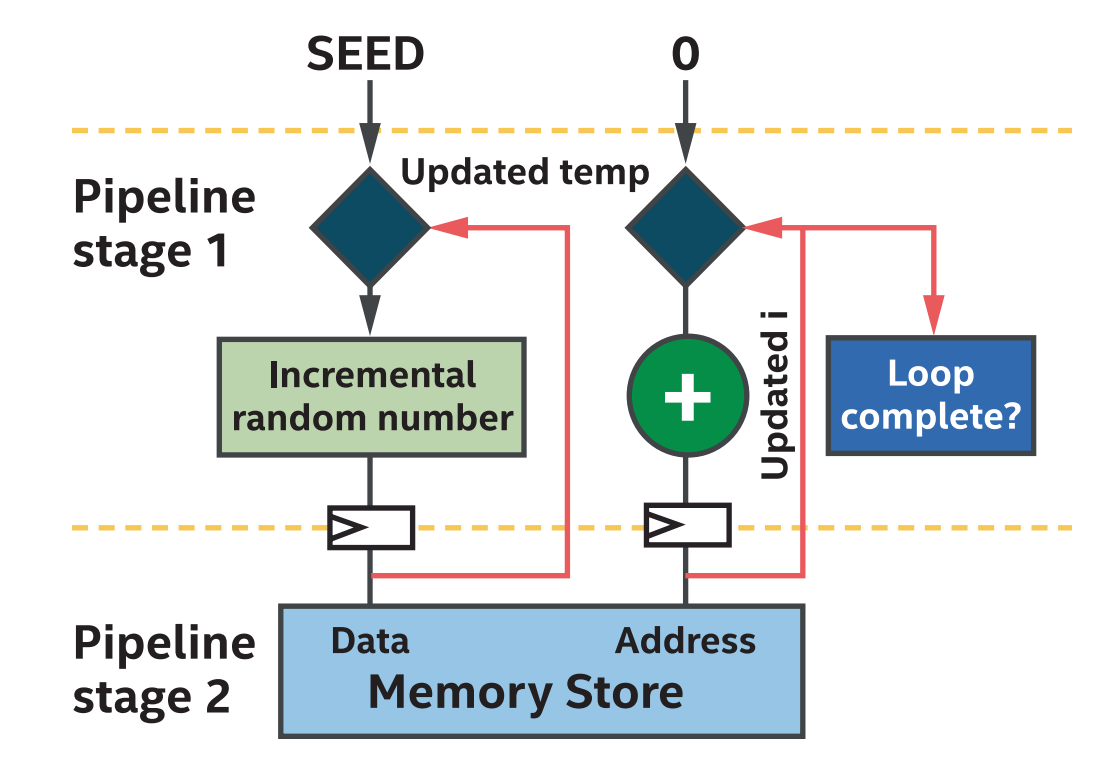
\includegraphics[width=1.0\textwidth]{content/chapter-17/images/20}
\end{center}

使用循环流水线,可以使循环的多次迭代执行重叠,即使使用循环携带的数据依赖项,循环迭代仍然可以用于用工作填充管道,从而实现高效利用。图17-26显示了循环迭代是如何在图17-25所示的同一个简单管道中重叠执行的。\par

\hspace*{\fill} \par %插入空行
图17-26 循环流水线同时处理多个循环迭代的部分
\begin{center}
	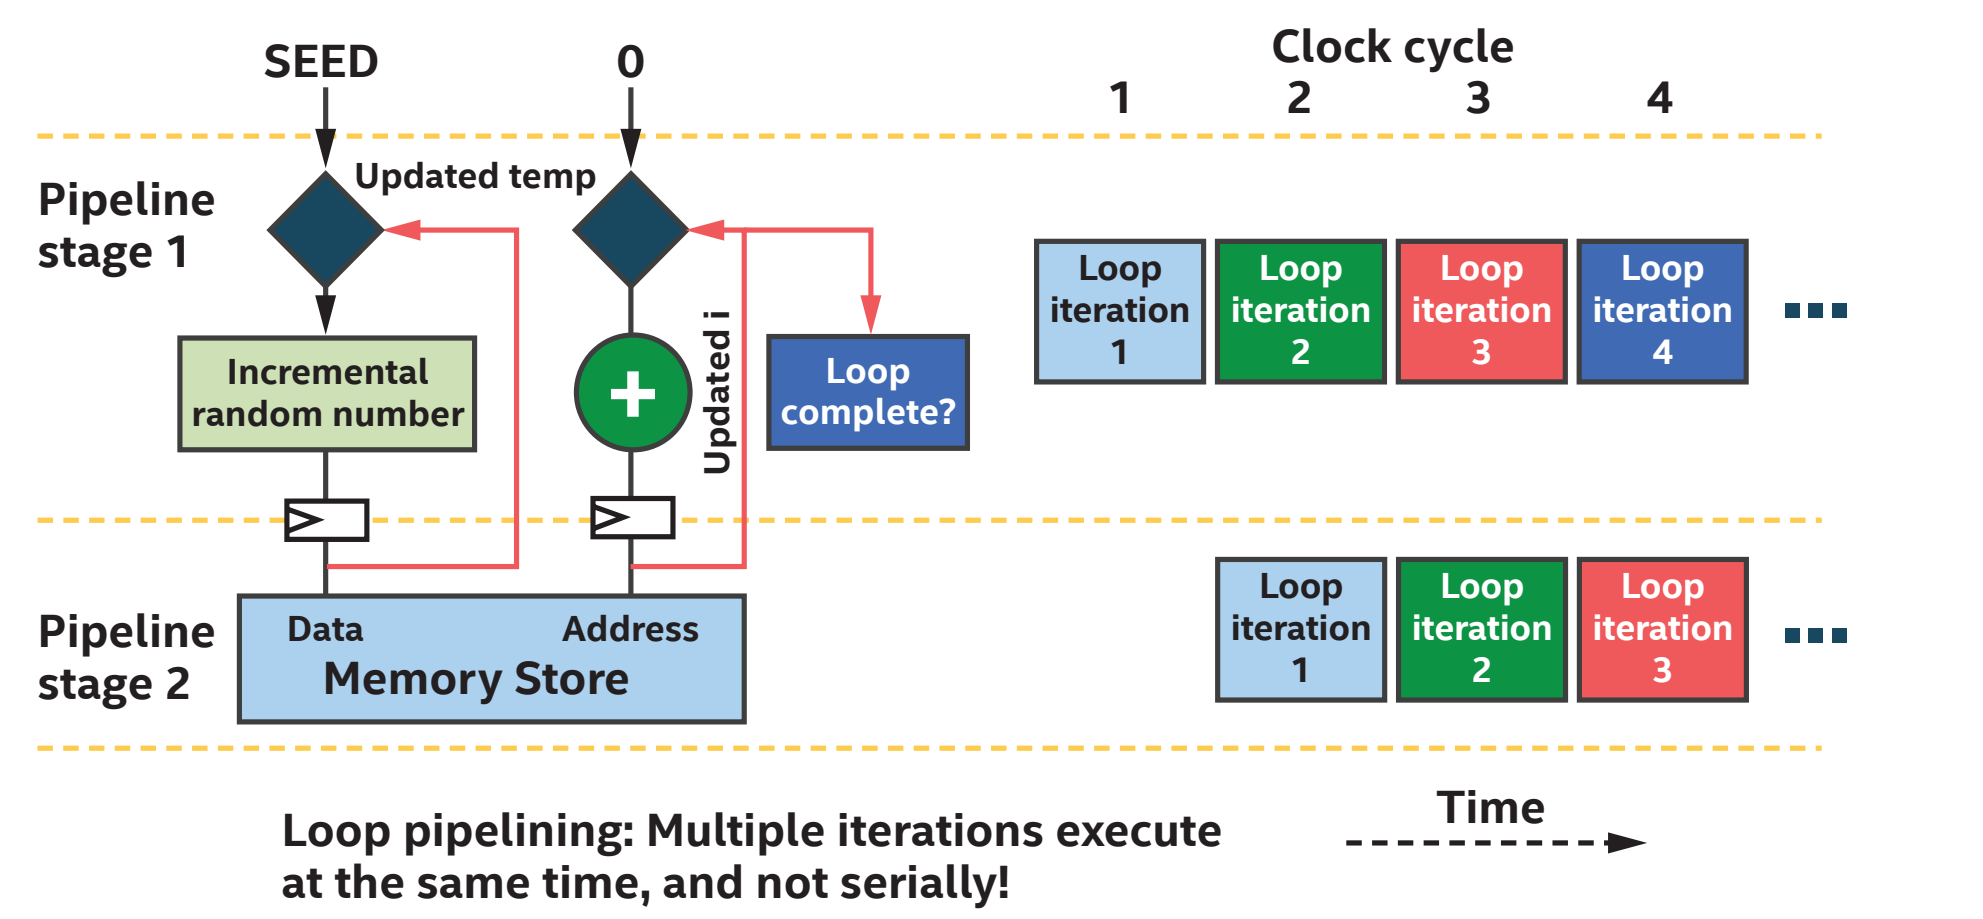
\includegraphics[width=1.0\textwidth]{content/chapter-17/images/21}
\end{center}

实际算法中,通常不可能在每个时钟周期中启动新的循环迭代,因为数据依赖可能需要多个时钟周期来计算。如果内存查找(特别是芯片外内存)处于依赖计算的关键路径上,则经常会出现这种情况。结果是一个管道,每N个时钟周期只能启动一个新的循环迭代,我们将其称为N个周期的起始间隔(II)。配置示例如图17-27所示。两个循环起始间隔(II)意味着一个新的循环迭代可以每秒钟开始一次,这导致管道阶段的次优占用。\par

\hspace*{\fill} \par %插入空行
图17-27 管道阶段的次优占用
\begin{center}
	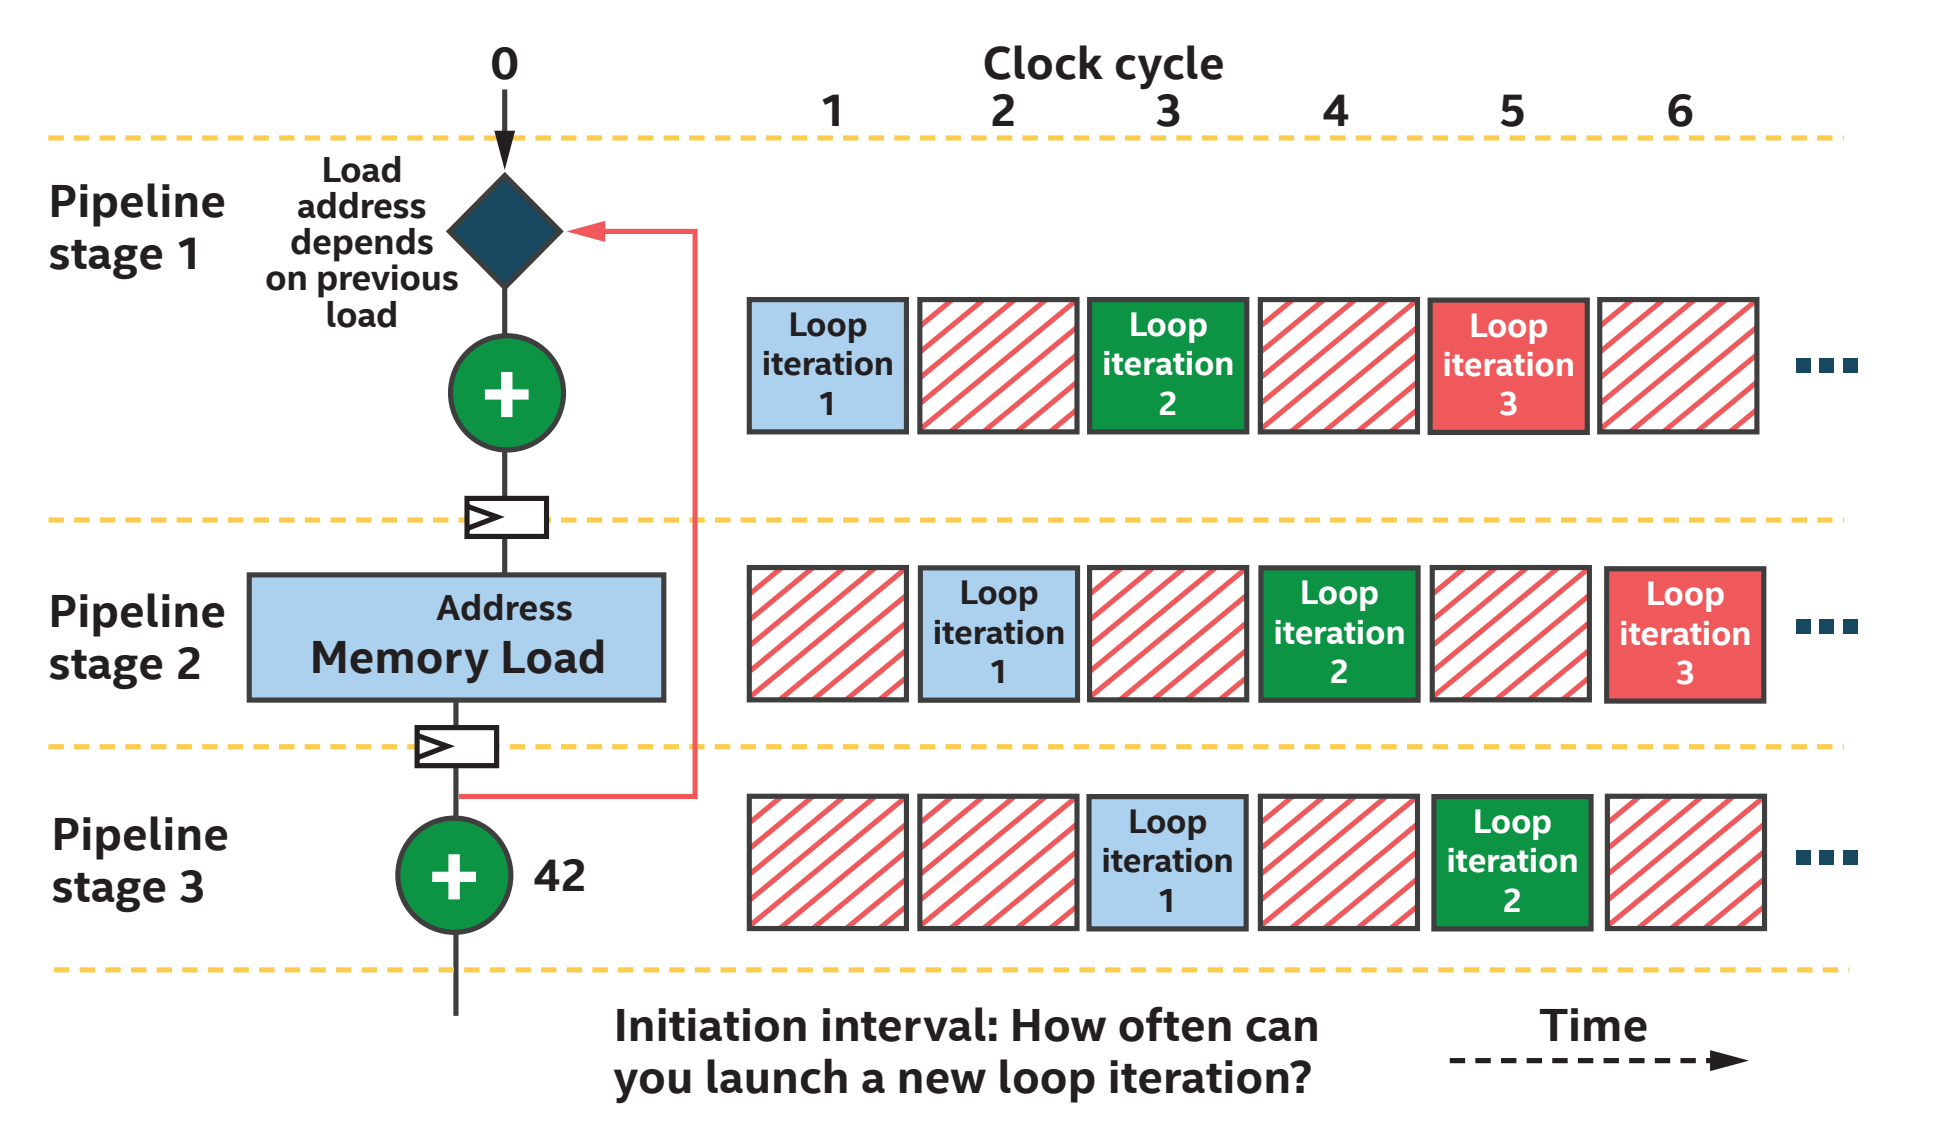
\includegraphics[width=1.0\textwidth]{content/chapter-17/images/22}
\end{center}

II大于1会导致流水线的效率低下,因为每个阶段的平均占用率都降低了。从图17-27中可以明显看出,II=2和管道阶段在很大比例(50\%!)的时间内没有使用。有很多方法可以改善这种情况。\par

编译器执行优化以尽可能地减少II,所以报告也会告诉我们每个循环的初始间隔是什么,并告诉我们为什么它大于1。基于报告在循环中重新构造计算通常可以减少II,我们可以进行编译器不允许的循环结构更改(因为是可观察的)。请阅读编译器报告,了解如何在特定情况下减少II。\par

降低II大于1的低效率的另一种方法是通过嵌套循环,它可以通过将具有II>1的内环迭代与外部循环迭代的交错来填充所有阶段。查看供应商文档和编译器报告,了解使用详细信息。\par

\hspace*{\fill} \par %插入空行
\textbf{管道}

空间和其他体系结构中的一个重要概念是先进先出(FIFO)缓冲区。FIFO之所以重要有很多原因,但在考虑编程时,有两个原因:\par

\begin{enumerate}
	\item 隐式控制信息与数据。这些信息告诉我们FIFO是空的还是满的,并且在将问题分解时非常有用。
	\item FIFO具有存储容量。在动态行为(如访问内存时的高可变延迟)时,可以更容易地实现性能。
\end{enumerate}

图17-28展示了一个简单的FIFO操作示例。\par

\hspace*{\fill} \par %插入空行
图17-28 一个FIFO的示例操作
\begin{center}
	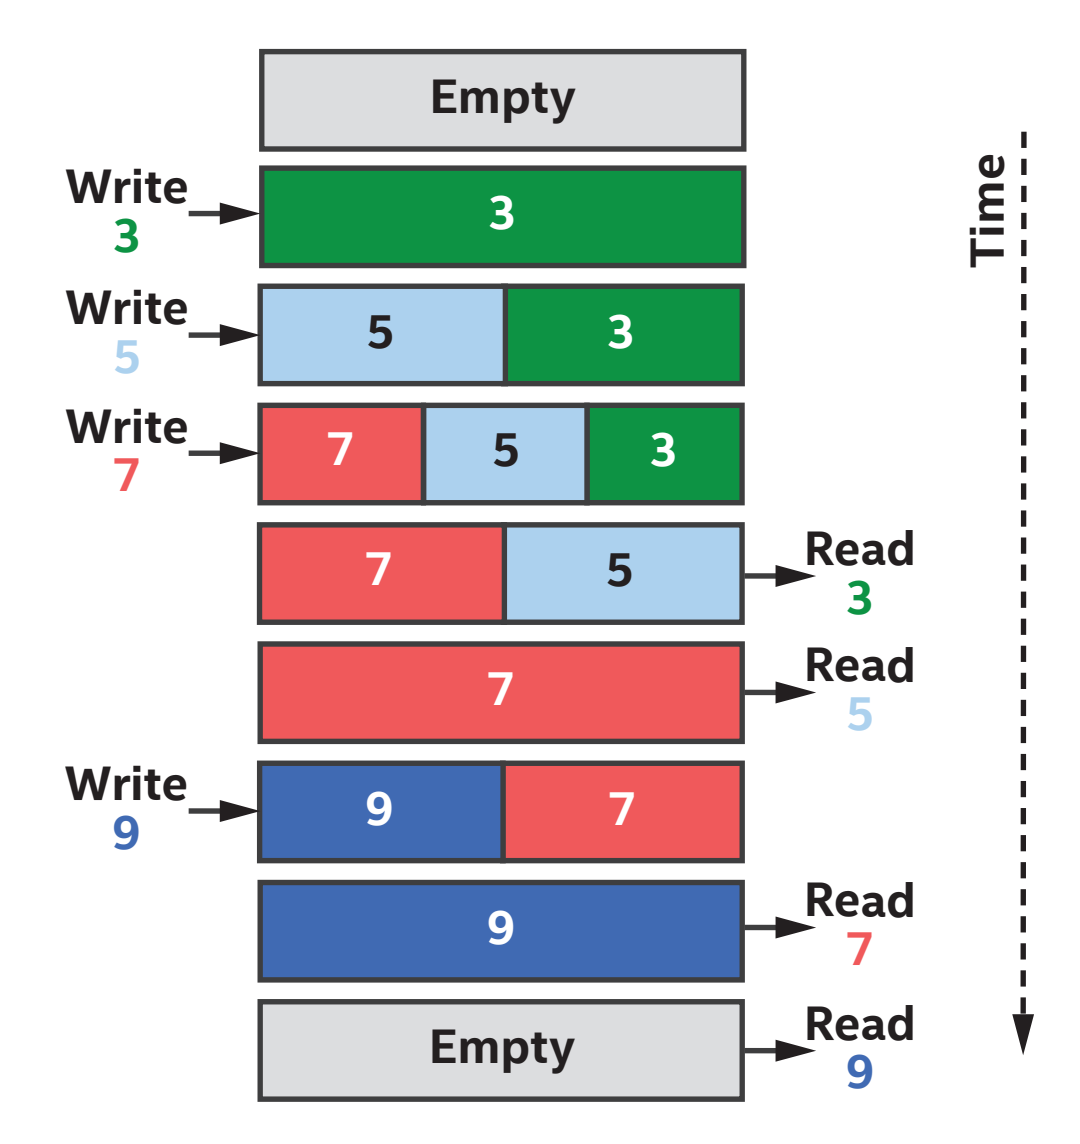
\includegraphics[width=1.0\textwidth]{content/chapter-17/images/23}
\end{center}

FIFO在DPC++中通过管道的特性对外使用。编写FPGA程序时,应该关心管道的原因是,管道允许我们将问题分解,以更模块化的方式关注开发和优化。还允许利用FPGA丰富的通信特性。如图17-29所示。\par

\hspace*{\fill} \par %插入空行
图17-29 管道简化了模块化设计和对硬件外设的访问
\begin{center}
	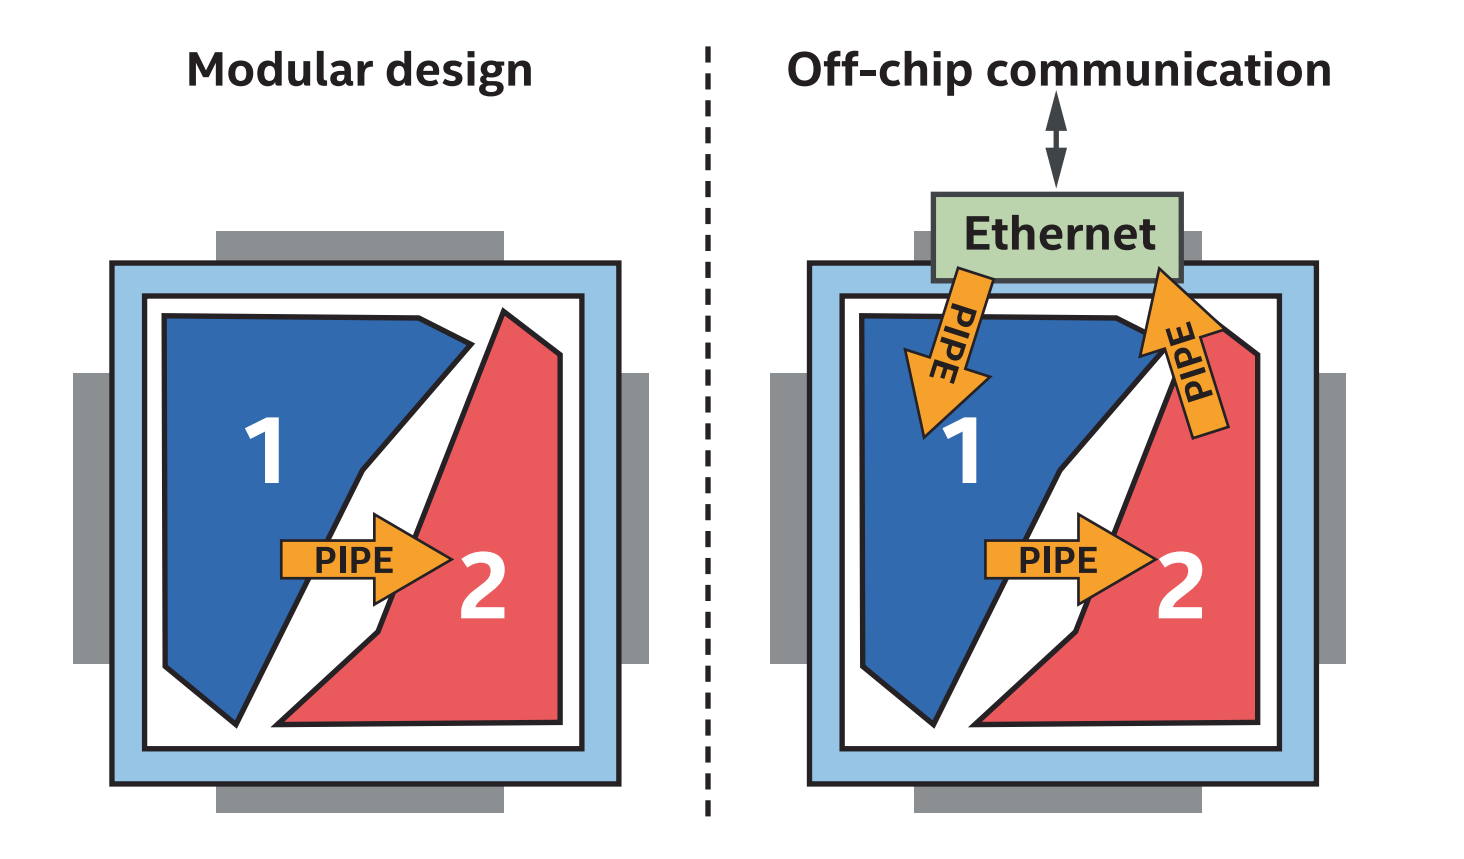
\includegraphics[width=1.0\textwidth]{content/chapter-17/images/24}
\end{center}

记住FPGA内核可以同时存在于设备上(在芯片的不同区域),在高效的设计中,内核的所有部分在每个时钟周期中都是活跃的。这意味着优化FPGA应用程序需要考虑内核或内核的各个部分如何相互交互,而管道提供了一个抽象来简化这一过程。\par

管道是使用FPGA上的片内存储器实现的FIFO,因此允许在运行的内核之间和内部进行通信,而无需将数据移动到片外存储器。可以提供廉价的通信,与管道(空/全信号)耦合的控制信息提供了轻量级的同步机制。\par

\begin{tcolorbox}[colback=blue!5!white,colframe=blue!75!black, title=我们需要管道吗?]
不使用管道也可以编写高效的内核。可以使用所有的FPGA资源,并在没有管道的情况下使用传统编程风格实现最大性能。但是对于大多数开发人员来说,编程和优化模块化空间设计更容易,而管道是实现这一目标的好方法。
\end{tcolorbox}

如图17-30所示,共有四种类型的管路。本节的其余部分中,将介绍第一种类型(内核间管道),因为它们可以说明什么是管道,以及如何使用管道。管道还可以在单个内核中与主机或输入/输出外设通信。请查看供应商文档,了解更多关于管道的形式和用途的信息。\par

\hspace*{\fill} \par %插入空行
图17-30 DPC++中管道连接的类型
\begin{center}
	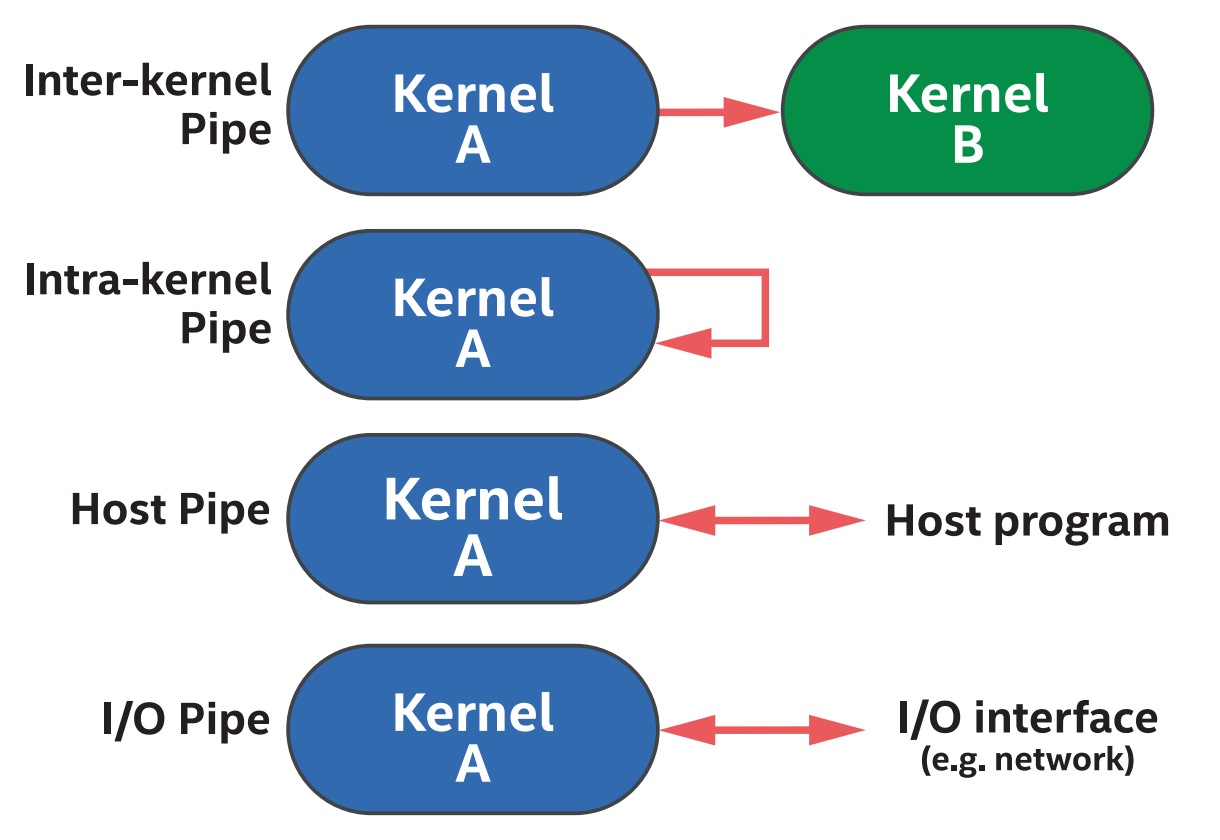
\includegraphics[width=1.0\textwidth]{content/chapter-17/images/25}
\end{center}

如图17-31所示。在这种情况下,有两个内核通过管道进行通信,每个读或写操作都以int为单位。\par

\hspace*{\fill} \par %插入空行
图17-31 两个内核之间的管道:(1)ND-range和(2)单个任务和一个循环
\begin{lstlisting}[caption={}]
// Create alias for pipe type so that consistent across uses
using my_pipe = pipe<class some_pipe, int>;

// ND-range kernel
Q.submit([&](handler& h) {
	auto A = accessor(B_in, h);
	
	h.parallel_for(count, [=](auto idx) {
		my_pipe::write( A[idx] );
	});
});

// Single_task kernel
Q.submit([&](handler& h) {
	auto A = accessor(B_out, h);
	
	h.single_task([=]() {
		for (int i=0; i < count; i++) {
			A[i] = my_pipe::read();
		}
	});
});
\end{lstlisting}

图17-31中有几点需要观察。首先,两个内核使用管道相互通信。如果内核之间没有访问器或事件依赖,DPC++运行时将同时执行,允许通过管道而不是完整的SYCL内存缓冲区或USM进行通信。\par

管道使用基于类型的方法进行标识,其中每个管道都使用管道类型的参数化进行标识,如图17-32所示。管道类型的参数化标识了特定的管道。对相同管道类型的读或写是对相同的FIFO。有三个模板参数一起定义了管道的类型,从而定义了管道的标识。\par

\hspace*{\fill} \par %插入空行
图17-32 参数化的管道类型
\begin{lstlisting}[caption={}]
template <typename name,
		  typename dataT,
		  size_t min_capacity = 0>
class pipe;
\end{lstlisting}

建议使用类型别名来定义管道类型,如图17-31中的第一行代码所示,以减少编程错误并提高代码可读性。\par

\begin{tcolorbox}[colback=red!5!white,colframe=red!75!black]
使用类型别名来标识管道。这简化了代码并防止意外的创建管道。
\end{tcolorbox}

管道有一个min\_capacity参数,它默认为0,这是自动选择,如果指定了,它保证至少有一定数量的单词可以写入管道,而不会读出任何单词。此参数在以下情况下有用\par

\begin{enumerate}
	\item 两个与管道通信的内核不会同时运行,需要管道中有足够的容量,让第一个内核在第二个内核开始运行并从管道中读取之前写入它的所有输出。
	\item 如果内核突然生成或消耗数据,那么向管道添加容量可以提供内核隔离,将它们解耦。例如,产生数据的内核可以继续写(直到管道容量满了),即使消耗数据的内核很忙,还没有准备好消耗任何东西。这提供了相对于其他内核执行的灵活性,仅以FPGA上的一些内存资源为代价。
\end{enumerate}

\hspace*{\fill} \par %插入空行
\textbf{阻塞和非阻塞管道访问}

像大多数FIFO接口一样,管道有两种类型的接口:阻塞和非阻塞。阻塞访问等待(阻塞/暂停执行!)操作成功,而非阻塞访问立即返回,并设置布尔值指示操作是否成功。\par

成功的定义很简单:如果正在从管道中读取数据,并且有可用数据可读(管道不是空的),则读取成功。如果正在写,而管道还没有满,则写入成功。图17-33显示了pipe类的两种访问成员函数形式。我们看到管道的成员函数允许对其进行写入或读取。对管道的访问可以是阻塞的,也可以是非阻塞的。\par

\hspace*{\fill} \par %插入空行
图17-33 允许写入或读取管道的成员函数
\begin{lstlisting}[caption={}]
// Blocking
T read();
void write( const T &data );

// Non-blocking
T read( bool &success_code );
void write( const T &data, bool &success_code ); 
\end{lstlisting}

阻塞访问和非阻塞访问都有用,这取决于我们的应用程序试图实现什么。如果内核在从管道中读取数据之前不能做更多的工作,那么使用阻塞读取可能是有意义的。如果内核希望从一组管道中的任何一个读取数据,但它不确定哪个管道可能有可用的数据,那么使用非阻塞调用从管道读取数据更有意义。内核可以从管道中读取数据并处理数据(如果有数据),但如果管道是空的,它可以继续,尝试从可能有可用数据的下一个管道中读取数据。\par

\hspace*{\fill} \par %插入空行
\textbf{有关管道的更多信息}

这一章中,只能粗略地了解管道,但是现在应该对它有一个了解,以及了解了如何使用它们的基本知识。FPGA供应商文档提供了更多的信息和在不同类型应用程序中使用的许例,因此如果认为管道与特定需求相关,应该先查看这些文档。\par

\hspace*{\fill} \par %插入空行
\textbf{自定义内存系统}

为大多数加速器编程时,大部分优化工作都花在提高内存访问的效率上。FPGA设计也是如此,特别是当输入和输出数据通过芯片外存储器时。\par

FPGA上的内存访问值得优化有两个主要原因:\par

\begin{enumerate}
	\item 减少所需的带宽,特别是在带宽利用率低的情况下
	\item 修改内存的访问模式,避免流水线中的停顿
\end{enumerate}

在流水线中,有必要简单谈一下暂停。编译器内置了读取或写入特定类型内存所需的时间的假设,并相应地优化和平衡了管道,在进程中隐藏了内存延迟。但是,如果以一种低效的方式访问内存,就会引入更长的延迟,并作为管道中的副产品停滞不前,早期的阶段无法进行进度执行,因为等待,管道阶段阻塞了(例如,内存访问)。如图17-34所示,超过负载的管道停止工作。\par

\hspace*{\fill} \par %插入空行
图17-34 内存停滞也会导致流水线阶段停滞
\begin{center}
	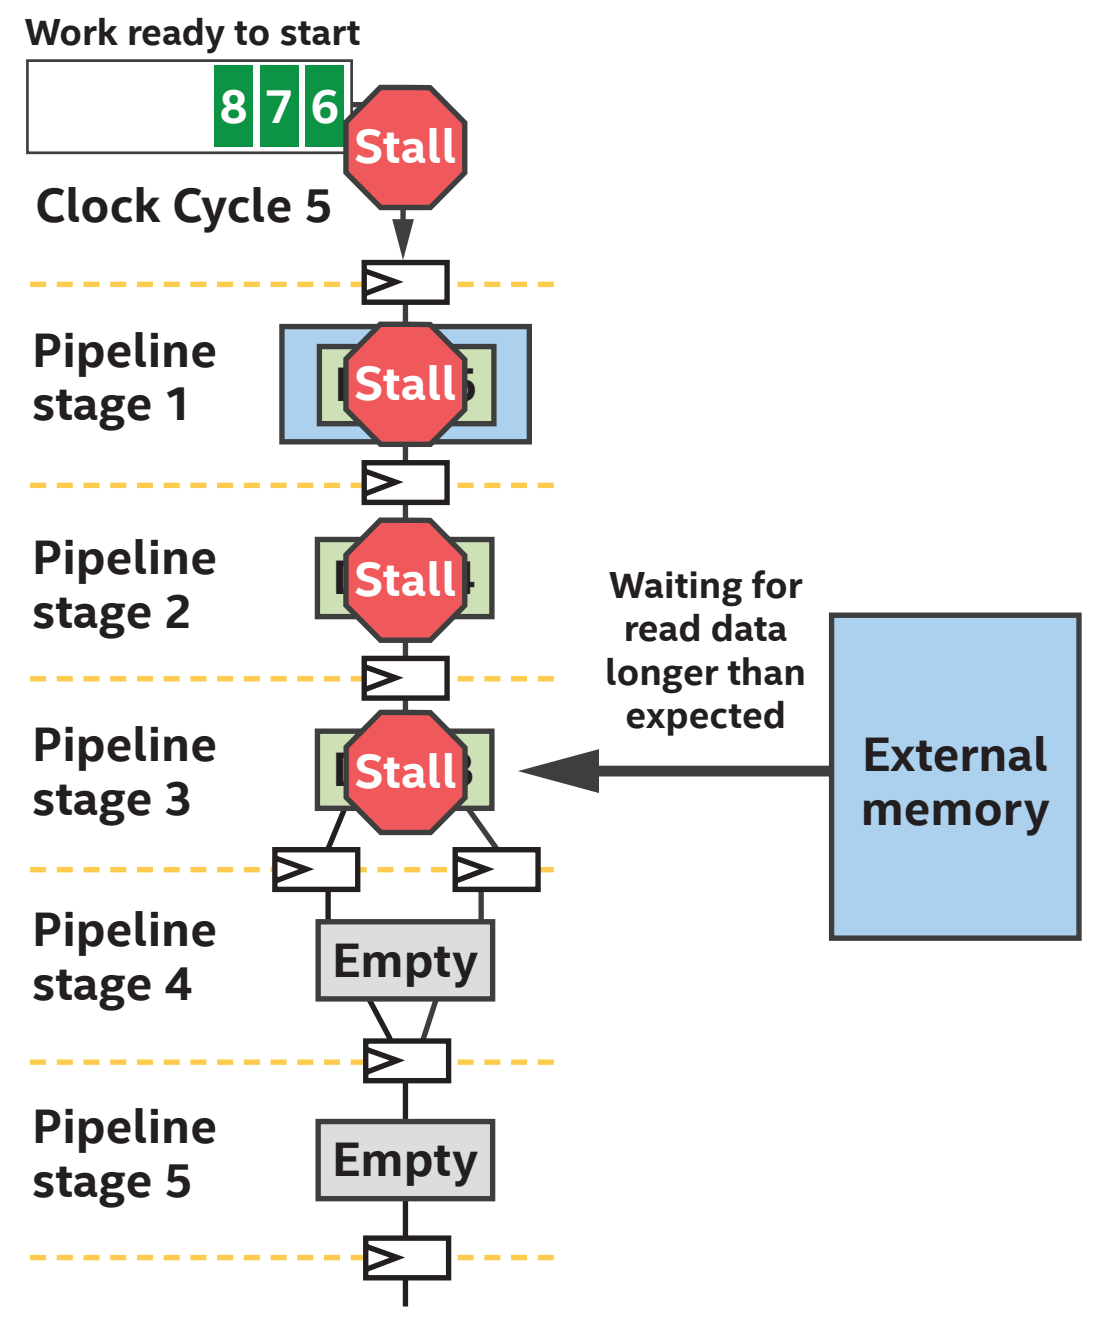
\includegraphics[width=1.0\textwidth]{content/chapter-17/images/26}
\end{center}

可以在几个方面执行内存系统优化。编译器报告是了解编译器为实现了什么,以及哪些可能值得调整或改进的重要指南。在这里列出了一些优化主题,以突出显示可供使用的自由度。优化通常可以通过显式控制和修改代码,让编译器推断想要的结构来实现。编译器静态报告和供应商文档,是内存系统优化的关键,有时在硬件执行期间与分析工具结合使用,以捕获实际的内存行为,用于验证或优化的最后阶段。\par

\begin{enumerate}
	\item 静态合并:编译器可以将内存访问合并为更小、更宽的访问。这降低了存储系统的复杂性,包括流水线中的负载或存储单元的数量、存储系统上的端口、仲裁网络的大小和复杂性,以及其他存储系统等。通常希望尽可能启用静态合并,这个可以通过编译器报告来确认。在内核中简化寻址逻辑有时就足以让编译器执行更激进的静态合并,所以总是检查编译器是否推断出我们所期望的报告!
	\item 内存访问风格:编译器为内存访问创建加载或存储单元,这些单元适合被访问的内存技术(例如,片上、DDR、HBM)和从源代码推断的访问模式(例如,流、动态合并/扩展,或可能从特定大小的缓存中获益)。编译器报告告诉我们推断了什么,并允许我们修改或添加控件到我们的代码,以提高性能。
	\item 内存系统结构:内存系统(包括芯片上和芯片外)可以具有由编译器实现的内存块结构和许多优化。可以使用许多控件和模式修改来控制这些结构和调优空间实现。
\end{enumerate}
















